\chapter{ผลการปฏิบัติงาน}
\label{chapter:result}

การการปฏิบัติงานสหกิจศึกษาที่ บริษัท ไซเจ็น ด้วยตำแหน่ง Full Stack Developer เป็นระยะเวลา 4 เดือน ตั้งแต่วันที่\StartDWork  จนถืงวันที่\EndDWork สามารถสรุปผลการปฏิบัติงานได้ดังนี้

\section{ผลการปฏิบัติงาน}

ฟังก์ชันหลักของเว็บแอพพลิเคชั่นประเมินความสามารถเบื้องต้นของผู้สมัครงาน สามารถทำงานได้ตามที่ได้ทำการออกแบบไว้ โดยสามารถส่งข้อสอบให้ผู้สมัครงานทำได้ผ่านอีเมล โดยอัติโนมัติ และสามารถตรวจข้อสอบแล้วสรุปผลออกมาเป็นคะแนนได้
โดยในฟังก์ชันหลักที่สร้างขึ้น จะถูกใช้ในส่วนต่อประสานกับผู้ใช้งานแต่ละหน้าต่อไปนี้

\subsection{หน้าเข้าสู่ระบบ}
\begin{figure}[H]
  \centering
  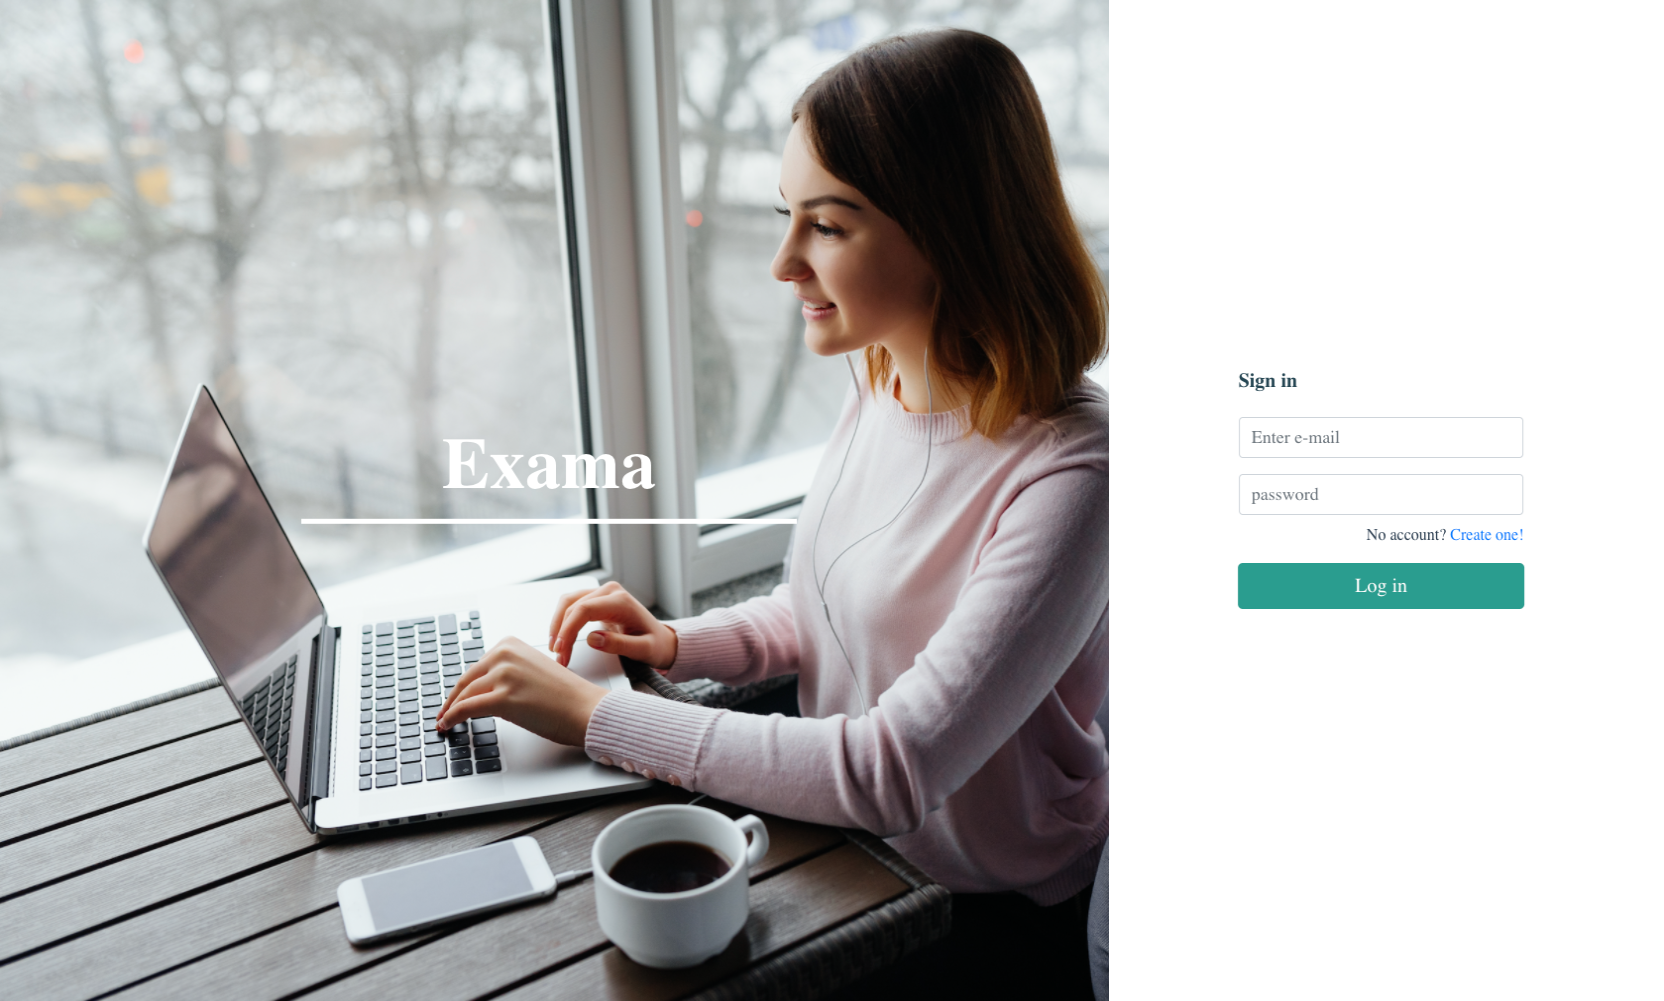
\includegraphics[width=1\columnwidth]{./page/login.png}
  \caption{แสดงหน้าเข้าสู่ระบบของเว็บแอพพลิเคชั่น}
  \label{Fig:Login}
\end{figure}
ในหน้าเข้าสู่ระบบประกอบด้วยฟังก์ชันการทำงานต่างๆ ดังนี้
\begin{itemize}
  \item Log in เพื่อเข้าสูระบบ
  \item Create one เพื่อสมัครสมาชิก
\end{itemize}

\subsection{หน้าสมัครสมาชิก}
\begin{figure}[H]
  \centering
  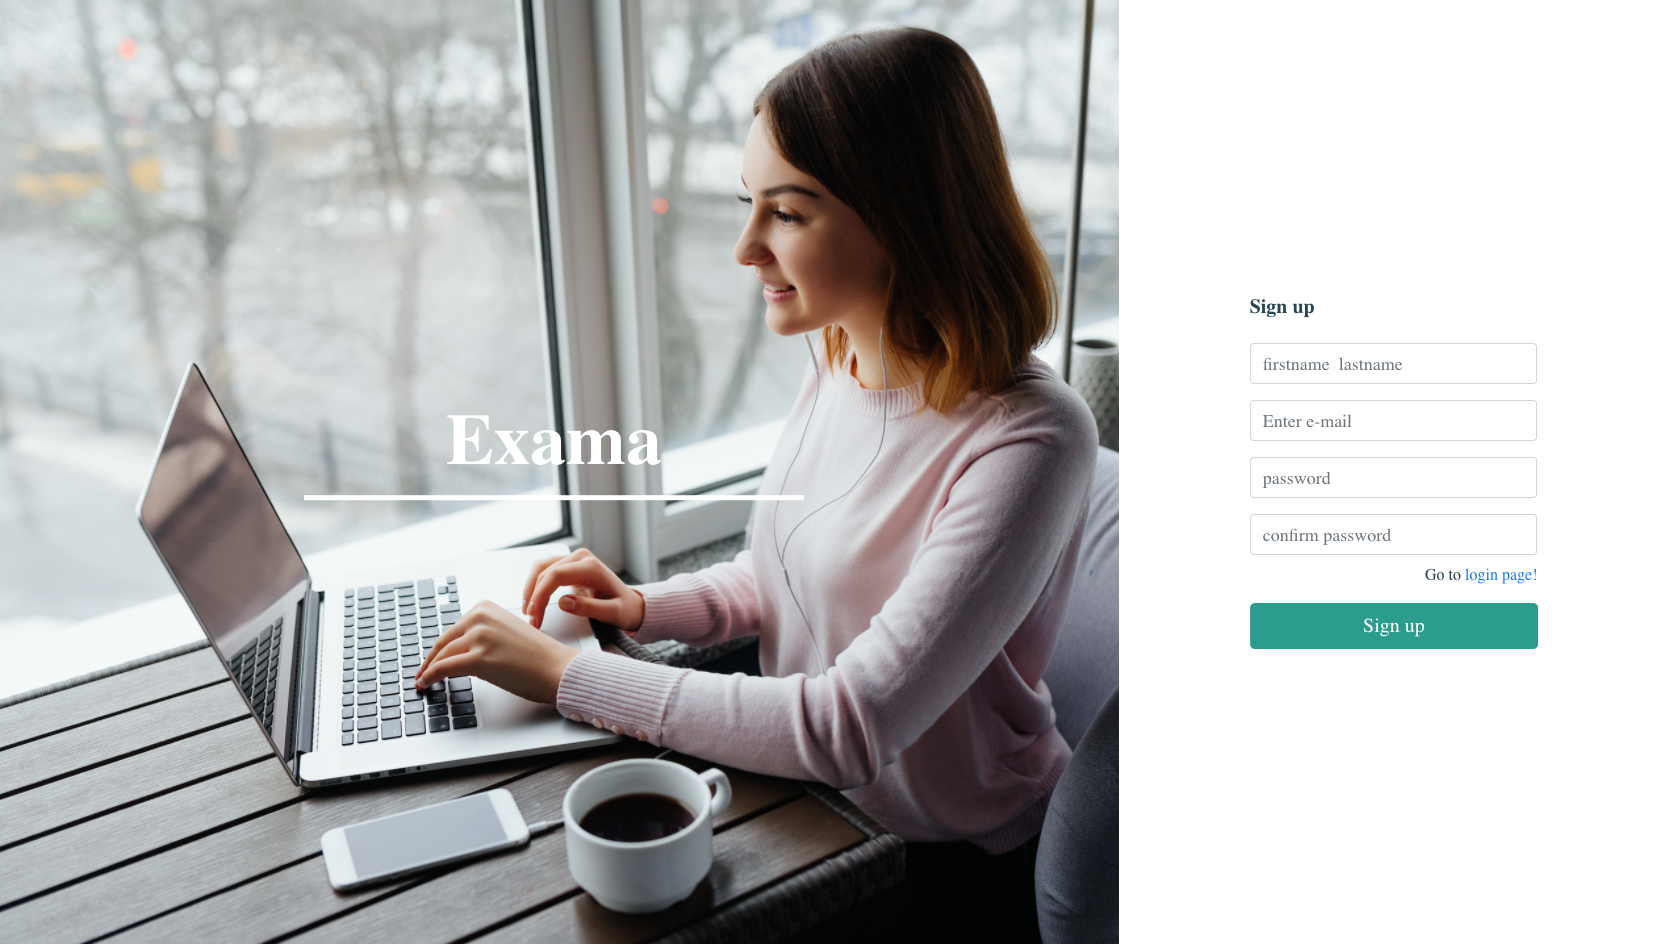
\includegraphics[width=1\columnwidth]{./page/singup.png}
  \caption{แสดงหน้าสมัครสมาชิกสู่ระบบของเว็บแอพพลิเคชั่น}
  \label{Fig:Register}
\end{figure}
ในหหน้าสมัครสมาชิกประกอบด้วยฟังก์ชันการทำงานต่างๆ ดังนี้
\begin{itemize}
  \item Sign up เพื่อสมัครสมาชิก ซึ่งจะมีอีเมลส่งไปที่ผู้สมัครสมาชิกเพื่อทำการยืนยันอีเมล หลังจากยืนยันอีเมลแล้ว ผู้ใช้งานถึงจะสามารถเข้าสู้ระบบได้
  \item Go to login page หากต้องการยกเลิกการสมัครสมาชิค
\end{itemize}

\subsection{หน้าหลัก}
\begin{figure}[H]
  \centering
  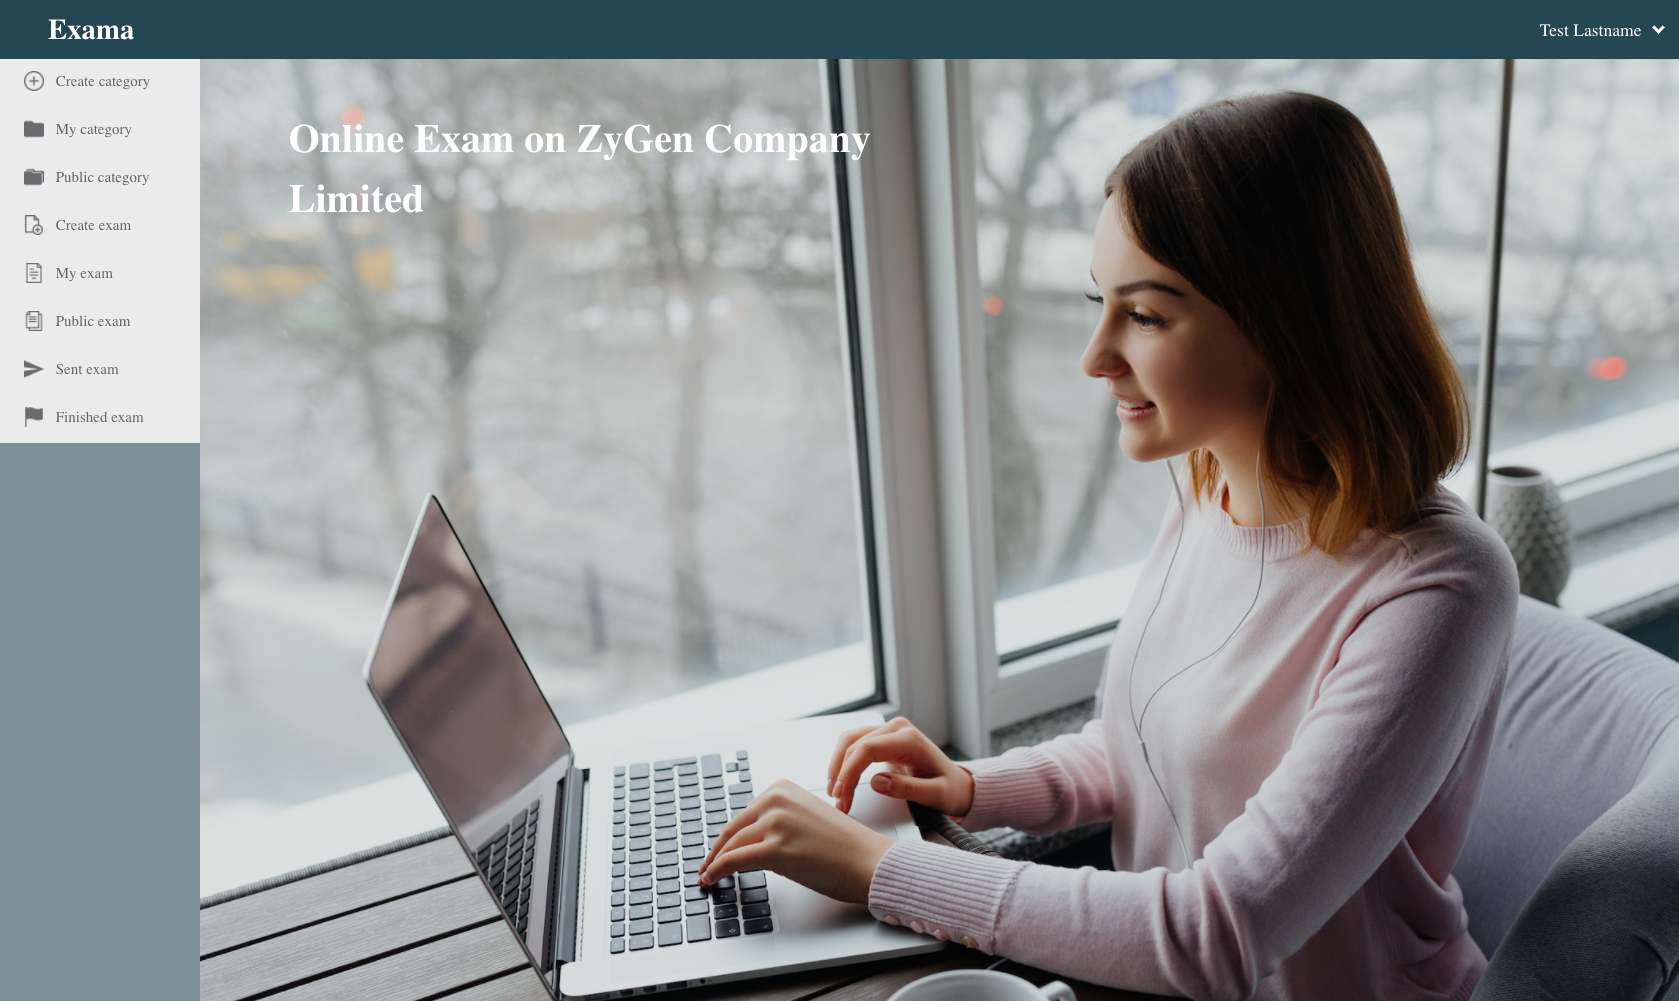
\includegraphics[width=1\columnwidth]{./page/home.png}
  \caption{แสดงหน้าหลักของเว็บแอพพลิเคชั่น}
  \label{Fig:Homepage}
\end{figure}
ในหหน้าหลักประกอบด้วยฟังก์ชันการทำงานต่างๆ ดังนี้
\begin{itemize}
  \item Side Navigation Menu เมนูเพื่อการเข้าถึงการทำงานต่างๆ
  \item logout เพื่อทำการออกสู่ระบบ โดยจะอยู่มุมบนซ้ายของหน้า หากนำเม้าส์ไปวางไว้ที่ชื่อของตนเอง
\end{itemize}

\subsection{หน้าสร้างหมวดหมู่คำถาม}
\begin{figure}[H]
  \centering
  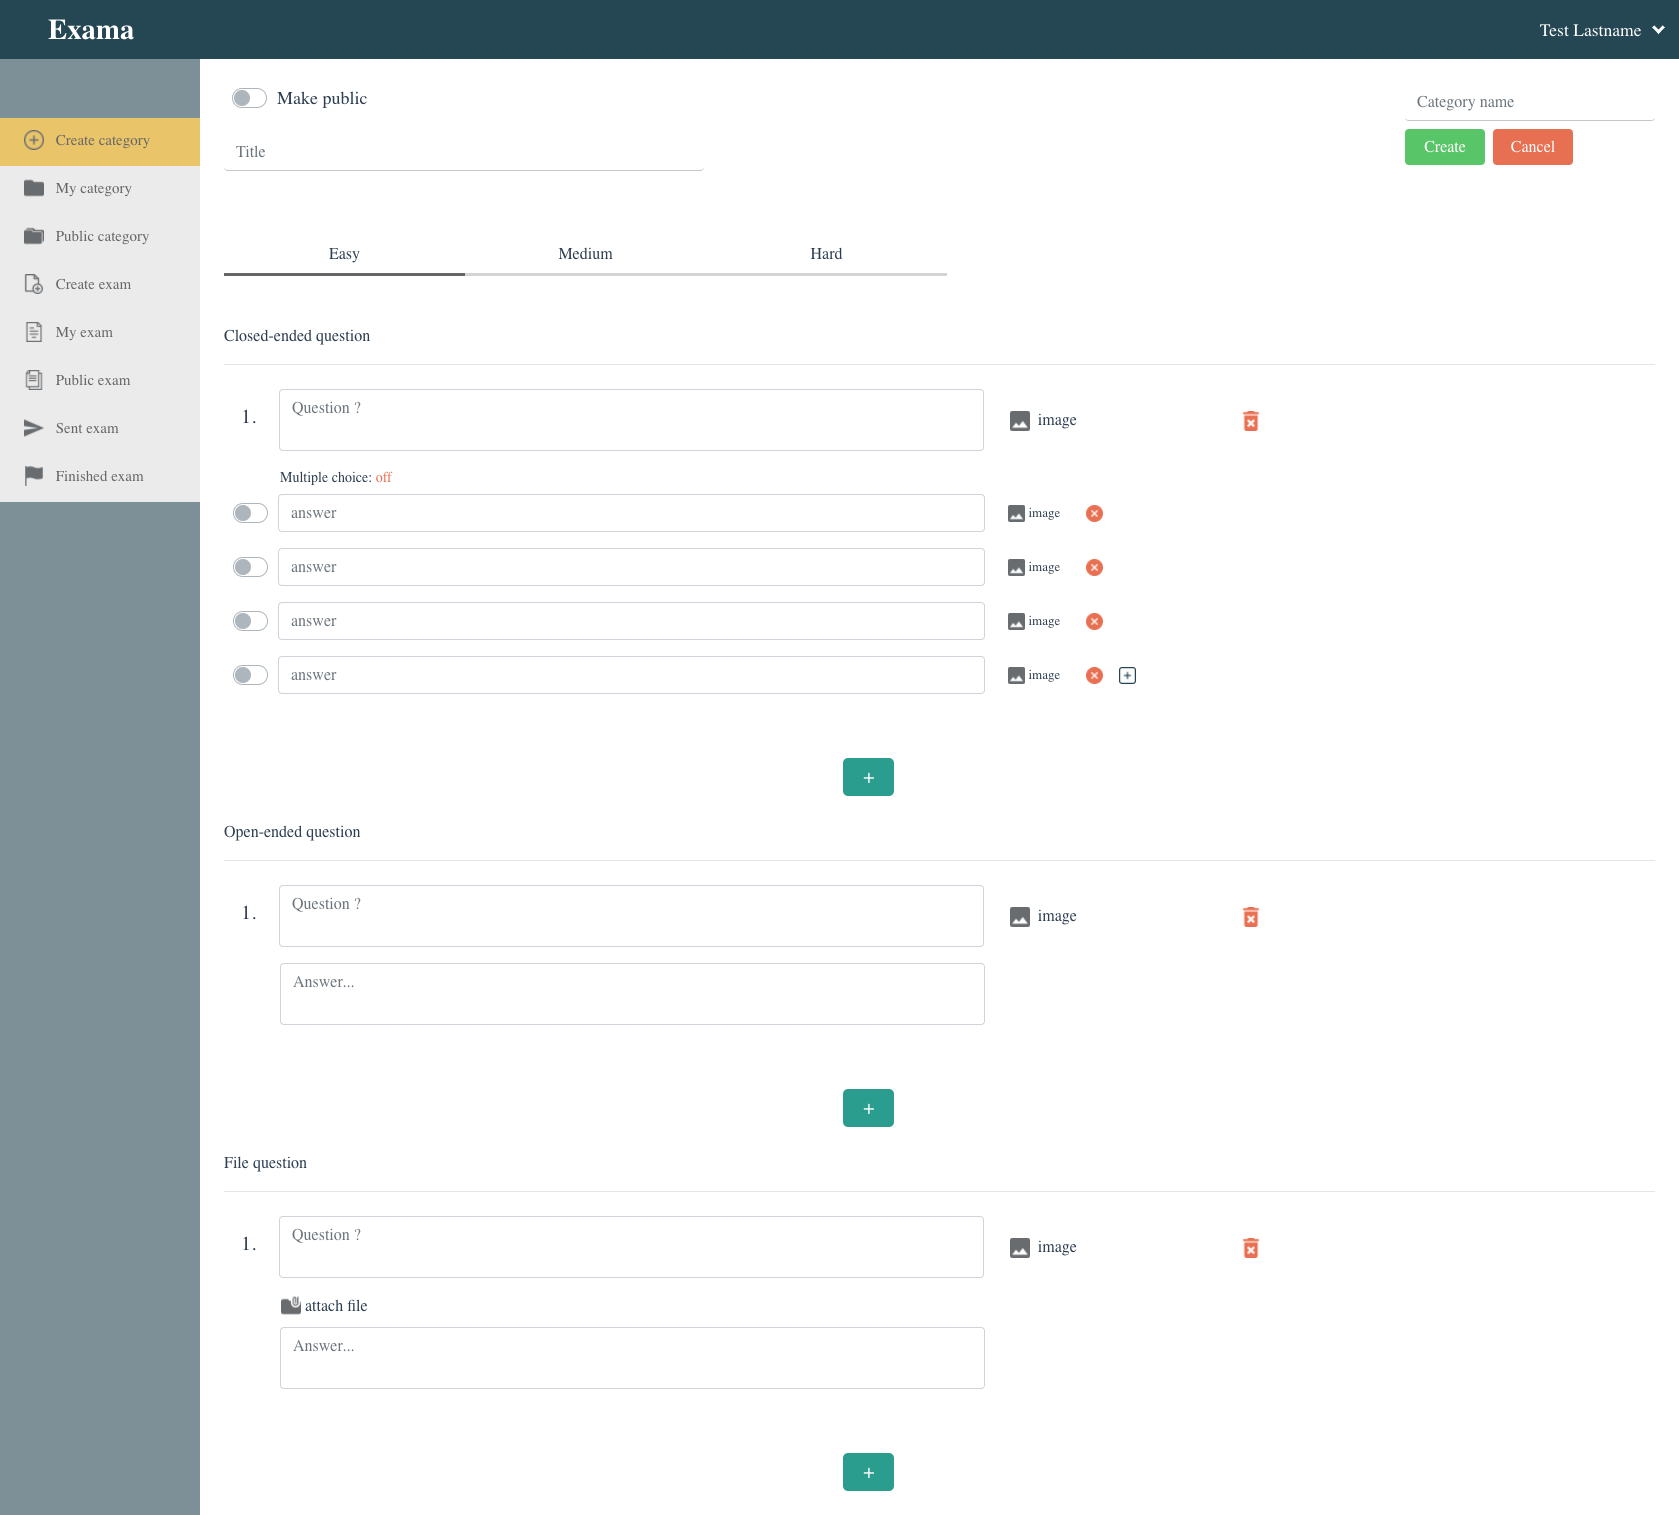
\includegraphics[width=1\columnwidth]{./page/createCat.png}
  \caption{แสดงหน้าสร้างหมวดหมู่คำถามของเว็บแอพพลิเคชั่น}
  \label{Fig:createCat}
\end{figure}
ในหหน้าสร้างหมวดหมู่คำถามประกอบด้วยฟังก์ชันการทำงานต่างๆ ดังนี้
\begin{itemize}
  \item ใส่รายละเอียดต่างๆของหมวดหมู่คำถาม
  \item สามารถกำหนดได้ว่าหมวดหมู่คำถามนี้ ต้องการเปิดเป็นสาธารณะให้ผู้อื่นใช้งานหรือไม่
  \item สามารถมีคำตามที่ถูกมากกว่า 1 ข้อได้
  \item สามารถเพิ่มตัวเลือกคำตอบของคำถามประเภทปรนัยได้
  \item สามารถ เพิ่ม ลบ หรือแก้ไขรูปภาพได้
  \item สามารถเพิ่มไฟล์ต่างๆได้
  \item สามารถลบคำถามออกได้
  \item สามารถกำหนดความยากข้อคำถามได้
  \item สามารถแนบไฟล์ในคำถามได้
  \item สามารถกำหนดเฉลยของคำถามได้
  \item สามารถเพิ่มคำถามได้
  \item สามารถป้องกันการกดเปลี่ยนหน้า, การปิดหน้า หรือการรีเฟรชหน้าได้ หากผู้ใช้งานทำการป้อนข้อมูลลงไปแล้ว
  \item สามารถยกเลิกการสร้างได้
\end{itemize}

\subsection{หน้าดูหมวดหมู่คำถามทั้งหมด}
\begin{figure}[H]
  \centering
  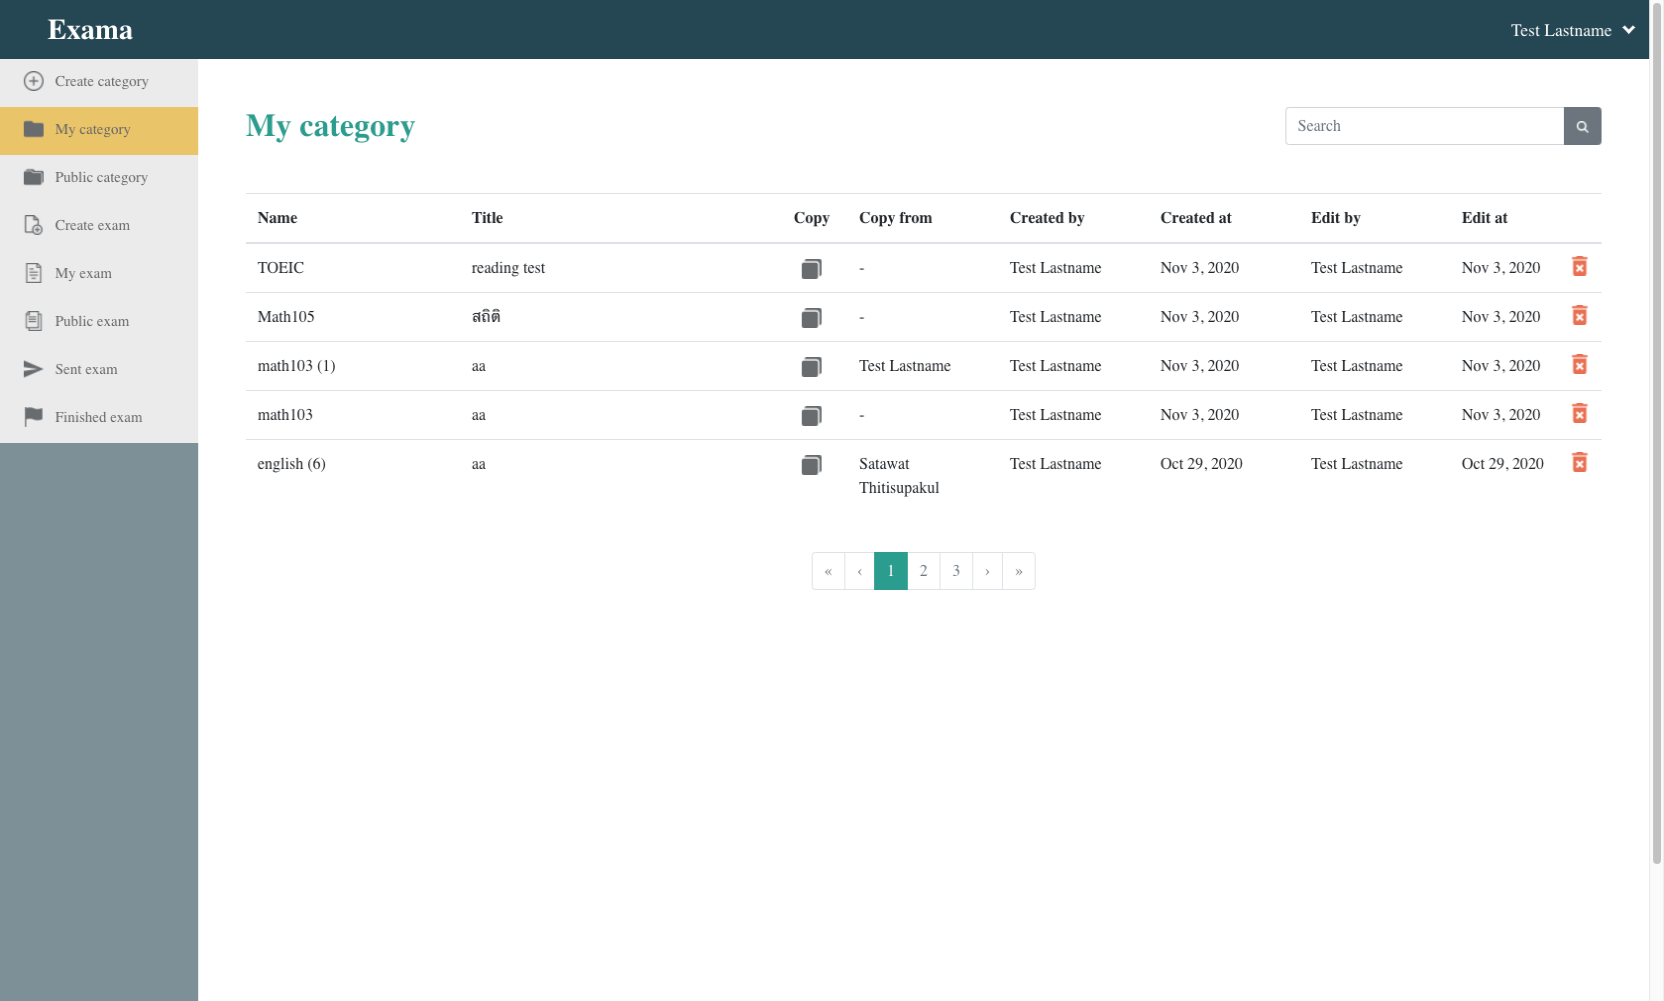
\includegraphics[width=1\columnwidth]{./page/myCat.png}
  \caption{แสดงหน้าดูหมวดหมู่คำถามทั้งหมดของเว็บแอพพลิเคชั่น}
  \label{Fig:myCat}
\end{figure}
ในหหน้าดูหมวดหมู่คำถามทั้งหมดประกอบด้วยฟังก์ชันการทำงานต่างๆ ดังนี้
\begin{itemize}
  \item สามารถค้นหา หมวดหมู่ที่ต้องการได้
  \item สามารถลบได้ หากไม่ถูกใช้ในข้อสอบ
  \item สามารถคัดลอกหมวดหมู่คำถามของตนเองได้
\end{itemize}

\subsection{หน้าแก้ไขหมวดหมู่คำถาม}
\begin{figure}[H]
  \centering
  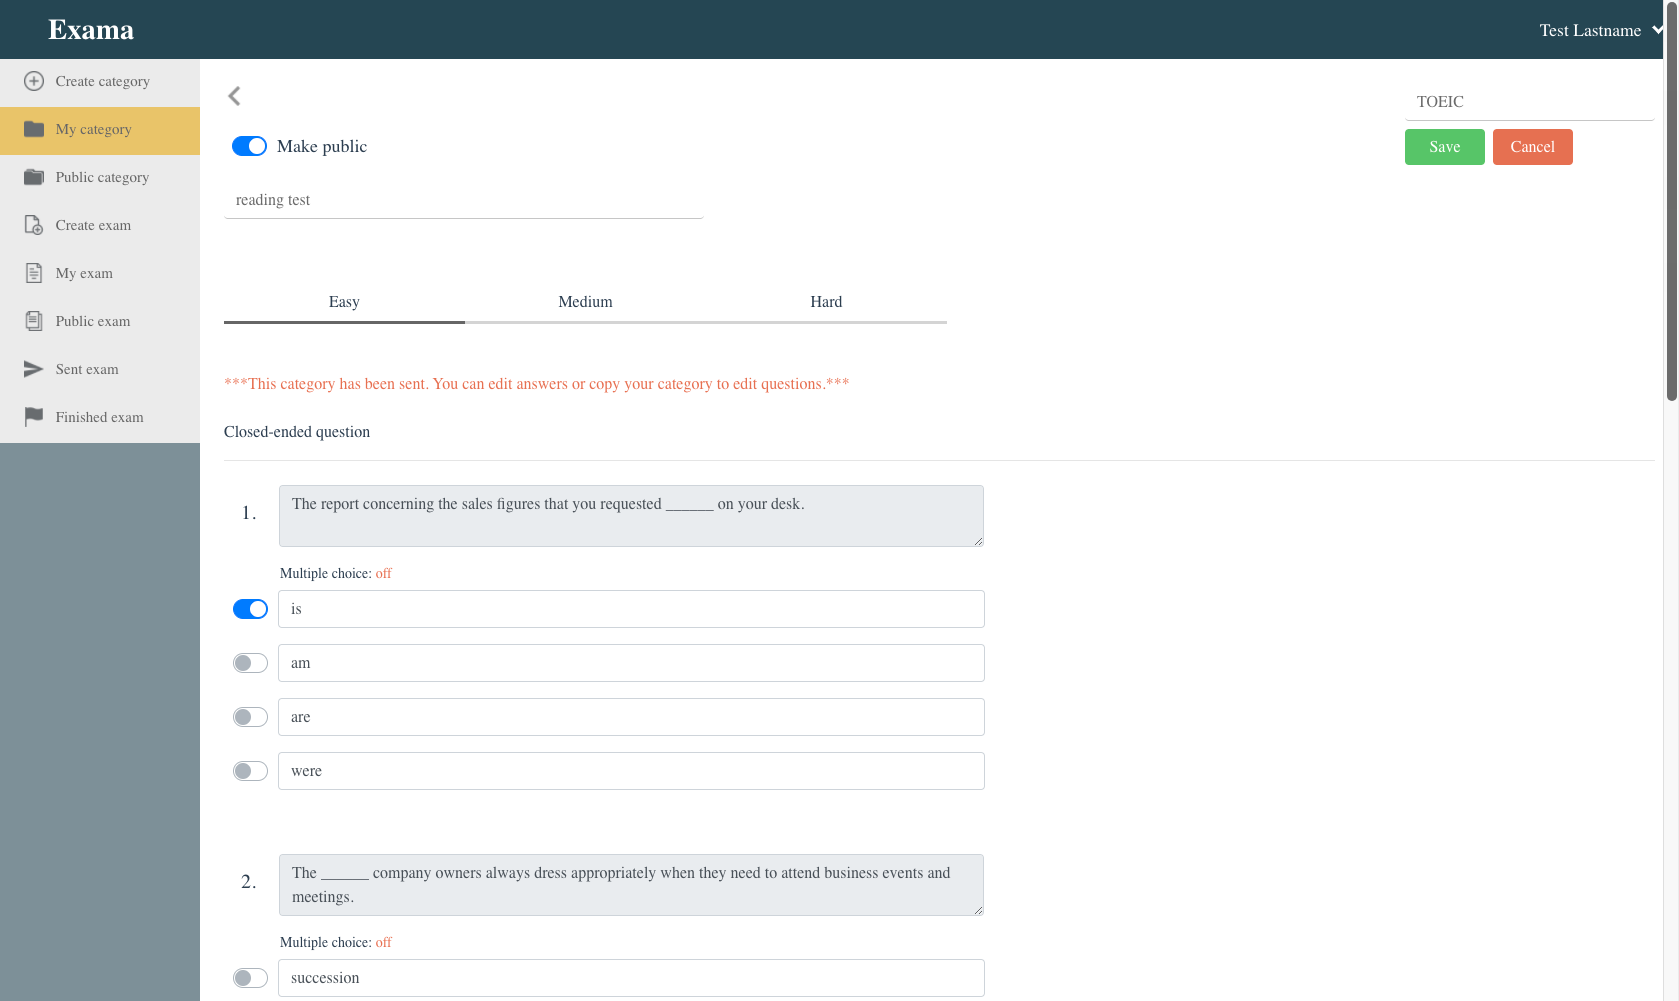
\includegraphics[width=1\columnwidth]{./page/catDetail.png}
  \caption{แสดงหน้าแก้ไขหมวดหมู่คำถามของเว็บแอพพลิเคชั่น}
  \label{Fig:myCatDetails}
\end{figure}
ในหน้าแก้ไขหมวดหมู่คำถามประกอบด้วยฟังก์ชันการทำงานต่างๆ ดังนี้
\begin{itemize}
  \item สามารถแก้ไขได้
  \item ถ้าหมวดหมู่คำถามนั้นนั้นมีการใช้ในข้อสอบ และถูกส่งให้ผู้สมัครงานแล้ว คำถามจะไม่สามารถแก้ไขได้ สามารถแก้ไขได้เพียงคำตอบดังรูป 4.6 เพื่อให้ผู้สมัครงานได้รับข้อสอบที่มีมาตรฐานเดียวกัน ถ้าต้องการแก้ไขส่วนอื่นๆให้ทำการคัดลอก เพื่อสร้างหมวดหมู่คำถามใหม่
  \item สามารถยกเลิกการแก้ไขได้
\end{itemize}

\subsection{หน้าดูหมวดหมู่คำถามที่เปิดเป็นสาธารณะ}
\begin{figure}[H]
  \centering
  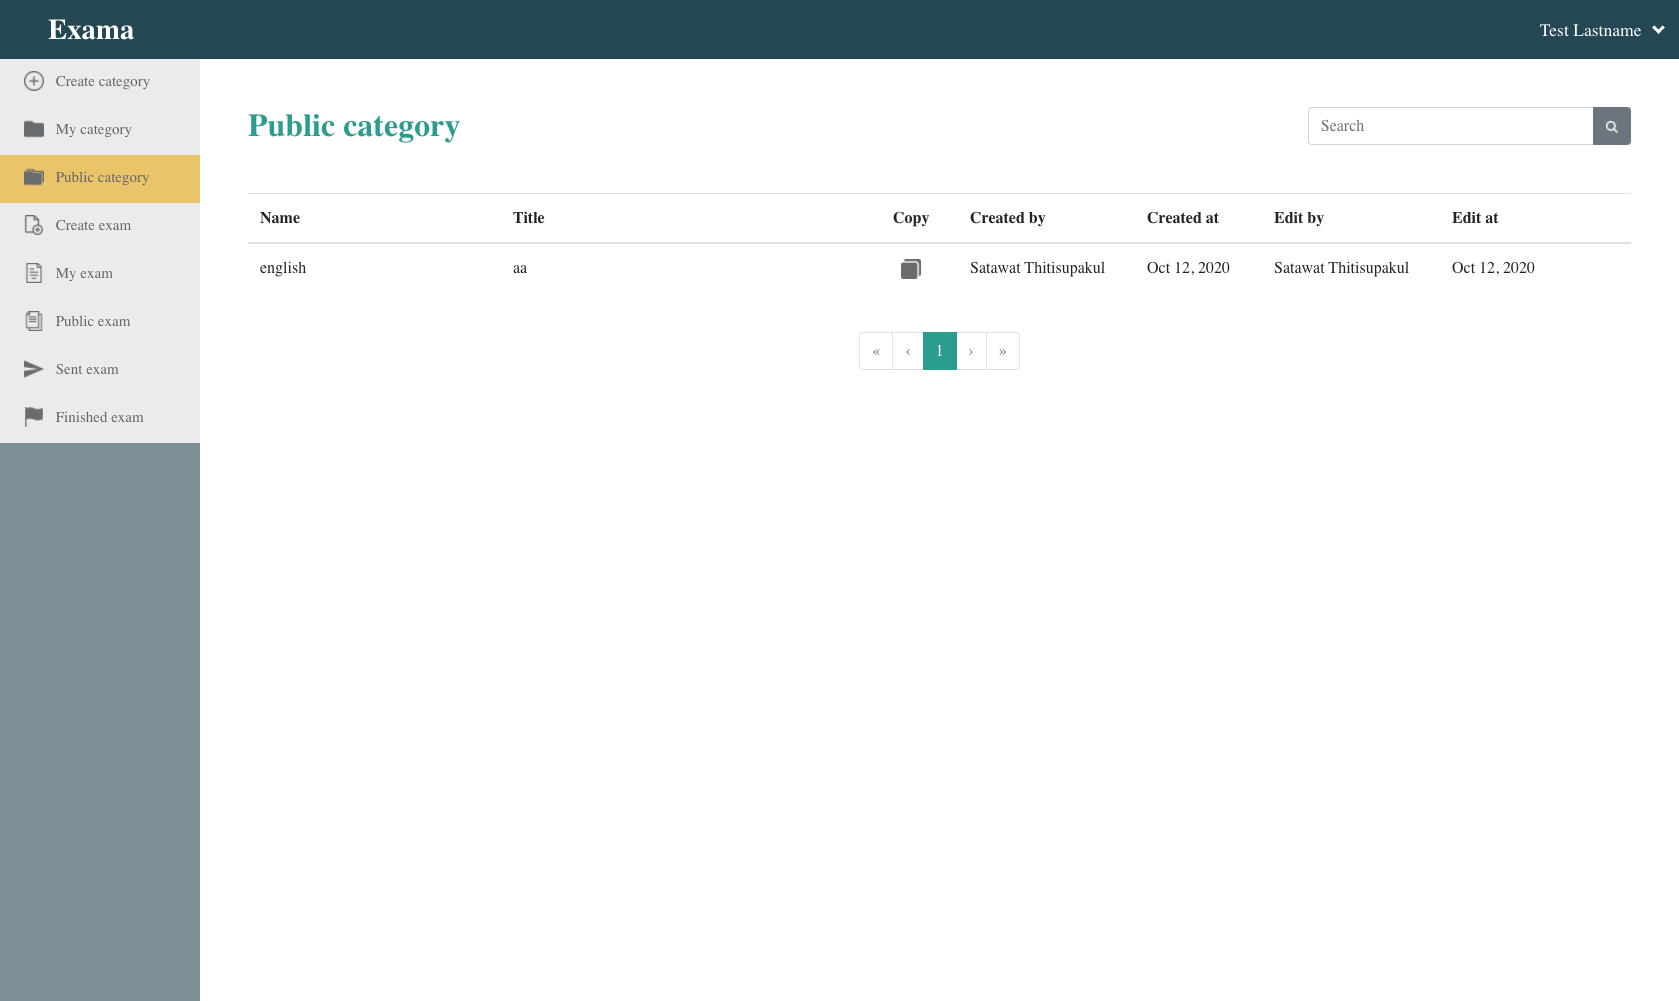
\includegraphics[width=1\columnwidth]{./page/pubCat.png}
  \caption{แสดงหน้าดูหมวดหมู่คำถามที่เปิดเป็นสาธารณะของเว็บแอพพลิเคชั่น}
  \label{Fig:pubCats}
\end{figure}
ในหน้าดูหมวดหมู่คำถามที่เปิดเป็นสาธารณะประกอบด้วยฟังก์ชันการทำงานต่างๆ ดังนี้
\begin{itemize}
  \item สามารถค้นหาได้
  \item สามารถคัดลอกหมวดหมู่คำถามเพื่อนำไปแก้ไขได้
  \item สามารถคลิกเข้าไปดูคำถามที่อยู่ในหมวดหมู่นั้นๆได้
\end{itemize}

\subsection{หน้าดูคำถามในหมวดหมู่คำถามที่เปิดเป็นสาธารณะ}
\begin{figure}[H]
  \centering
  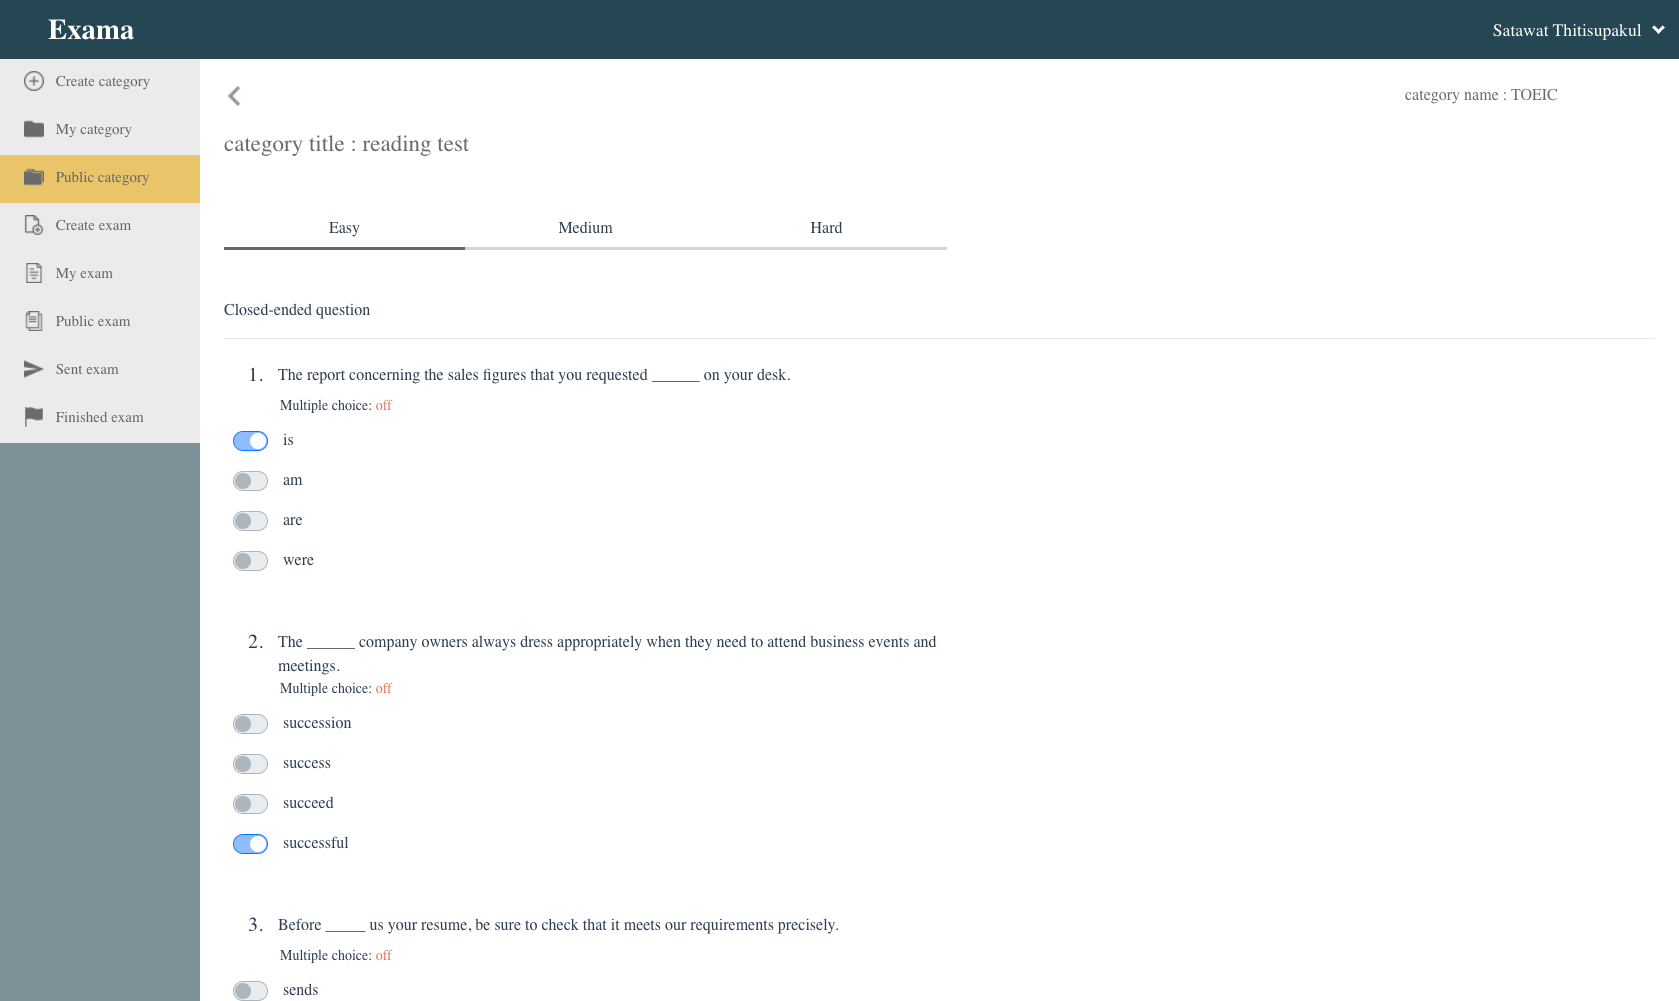
\includegraphics[width=1\columnwidth]{./page/pubCatDetails.png}
  \caption{แสดงหน้าดูคำถามในหมวดหมู่คำถามที่เปิดเป็นสาธารณะของเว็บแอพพลิเคชั่น}
  \label{Fig:pubCatDetail}
\end{figure}
ในหน้าดูคำถามในหมวดหมู่คำถามที่เปิดเป็นสาธารณะประกอบด้วยฟังก์ชันการทำงานต่างๆ ดังนี้
\begin{itemize}
  \item ดูรายละเอียด และคำถามในหมวดหมู่นั้น
\end{itemize}

\subsection{หน้าสร้างข้อสอบเพื่อใช้สำหรับผู้สมัครงาน}
\begin{figure}[H]
  \centering
  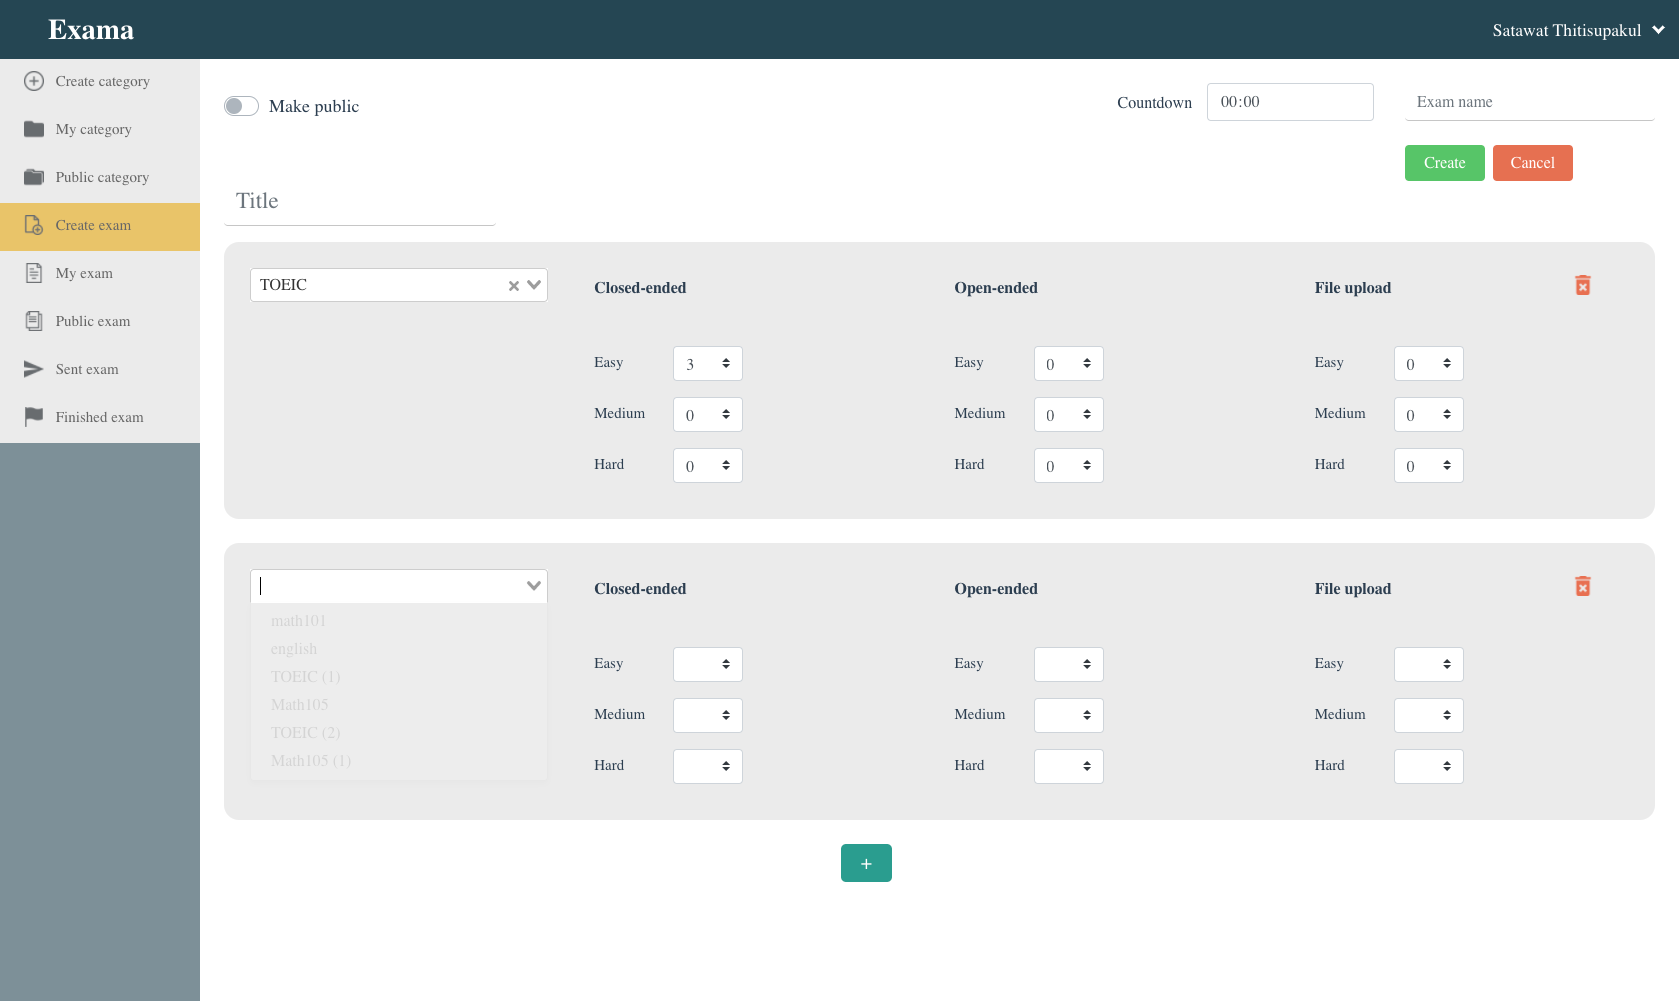
\includegraphics[width=1\columnwidth]{./page/createExam.png}
  \caption{แสดงหน้าสร้างข้อสอบเพื่อใช้สำหรับผู้สมัครงานของเว็บแอพพลิเคชั่น}
  \label{Fig:createExam}
\end{figure}
ในหน้าสร้างข้อสอบเพื่อใช้สำหรับผู้สมัครงานประกอบด้วยฟังก์ชันการทำงานต่างๆ ดังนี้
\begin{itemize}
    \item ใส่รายละเอียดต่างๆของข้อสอบ
    \item สามารถกำหนดได้ว่าข้อสอบนี้ ต้องการเปิดเป็นสาธารณะให้ผู้อื่นใช้งานหรือไม่ ชึ่งถ้าเปิดข้อสอบให้เป็นสาธารณะ หมวดหมู่คำถามที่ใช้ในข้อสอบ จะสามารถใช้ได้เฉพาะหมวดหมู่คำถามที่เป็นสาธารณะด้วยเท่านั้น
    \item สามารถพิมพ์ค้นหาหมวดหมู่ของคำถามที่ต้องการได้
    \item สามารถเลือกจำนวนข้อของแต่ละระดับความยาก และประเภทของข้อสอบได้
    \item สามารถเพิ่มหมวดหมู่ได้ ตามหมวดหมู่ที่มีทั้งหมด
    \item สามารถยกเลิกการสร้างได้
    \item สามารถป้องกันการกดเปลี่ยนหน้า,การปิดหน้าหรือการรีเฟรชหน้าได้หากผู้ใช้งานทําการป้อน ข้อมูลลงไปแล้ว
\end{itemize}

\subsection{หน้าดูข้อสอบของตนเอง}
\begin{figure}[H]
  \centering
  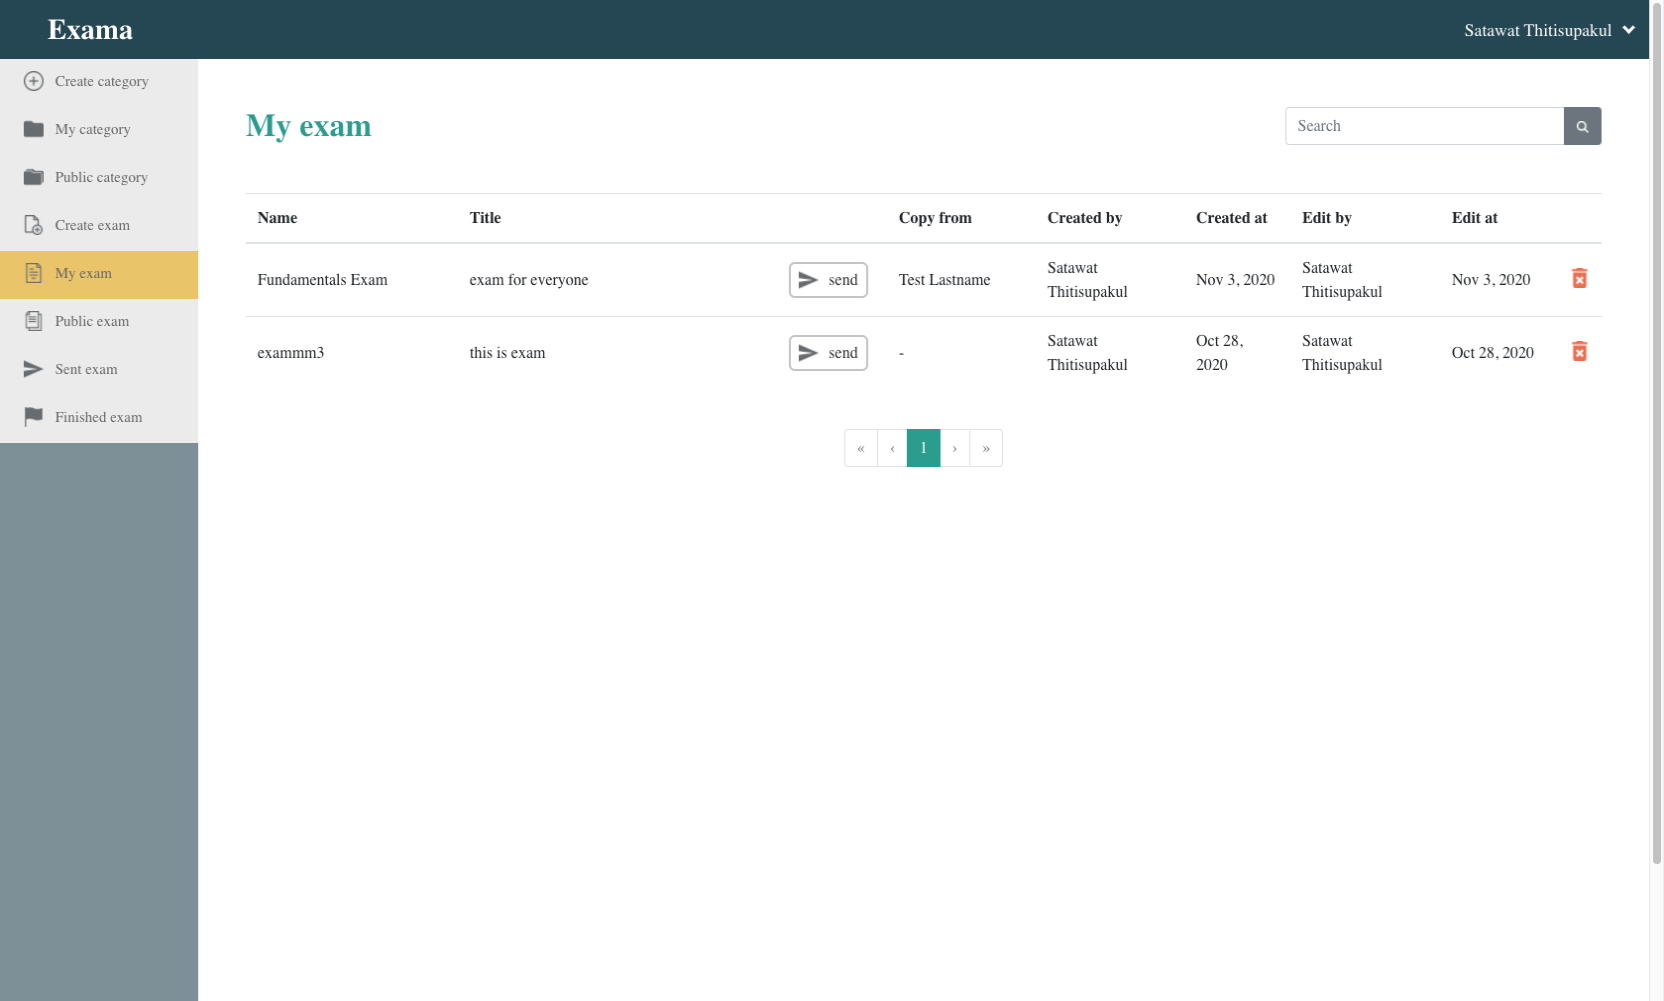
\includegraphics[width=1\columnwidth]{./page/myExam.png}
  \caption{แสดงหน้าดูข้อสอบตนเองของเว็บแอพพลิเคชั่น}
  \label{Fig:myExam}
\end{figure}
\begin{figure}[H]
    \centering
    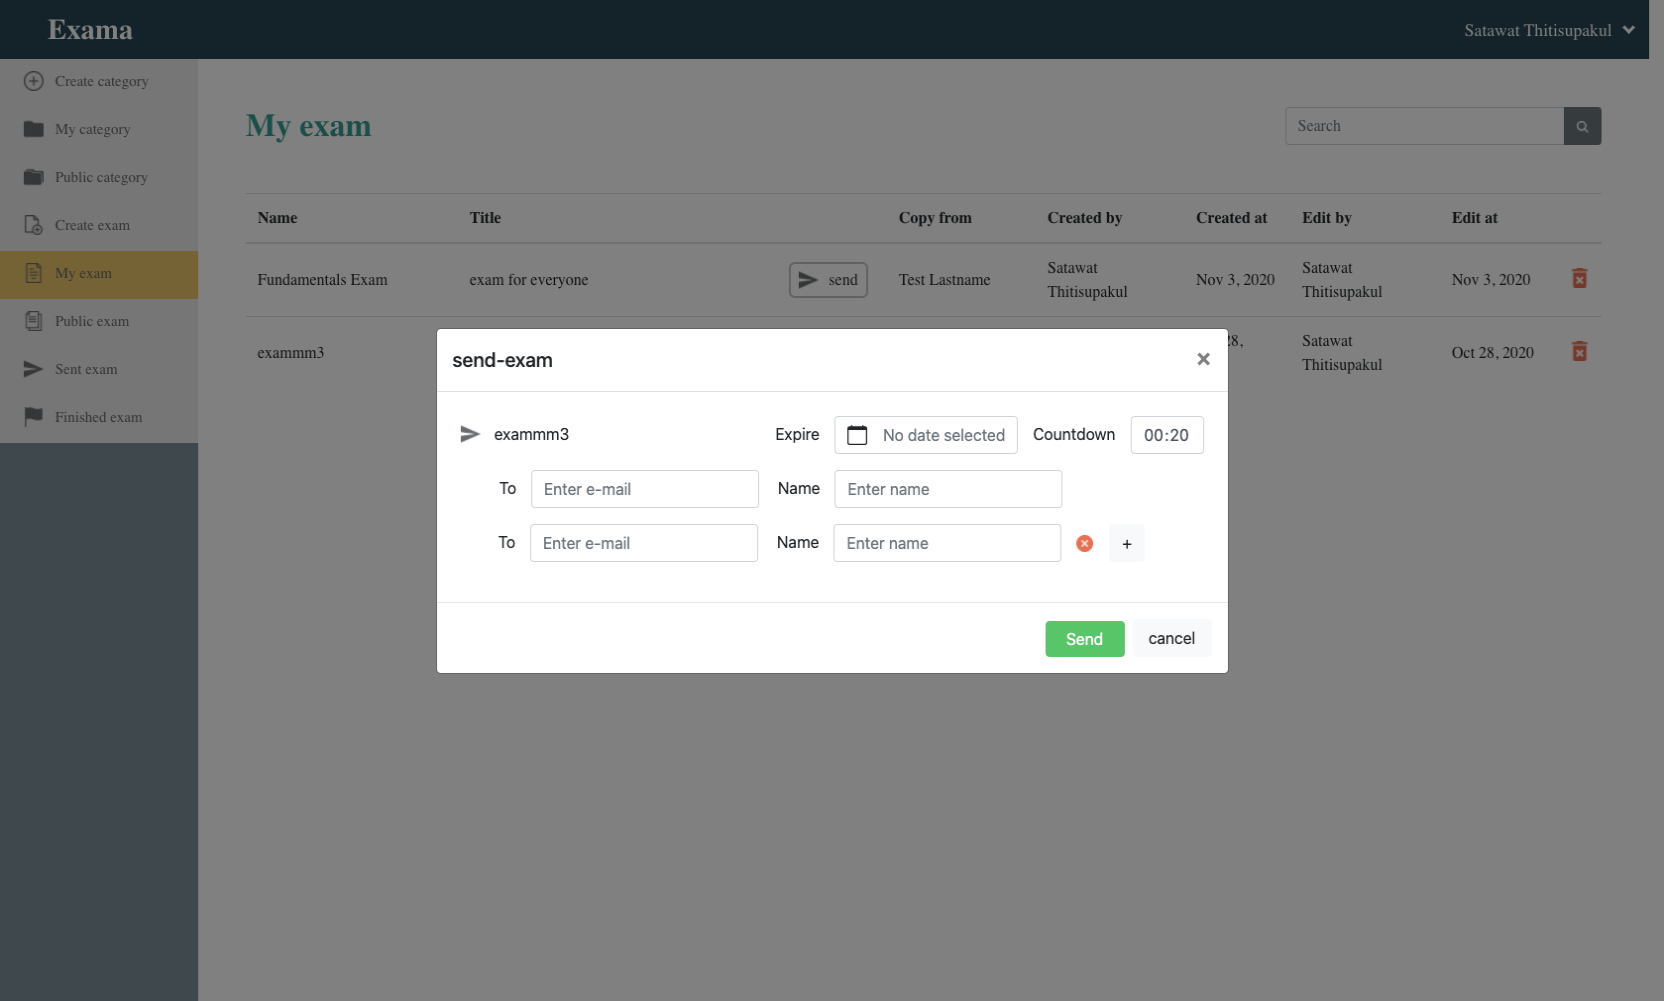
\includegraphics[width=1\columnwidth]{./page/sendExam.png}
    \caption{แสดงหน้าดูข้อสอบตนเองในขั้นตอนส่งข้อสอบให้ผู้สมัครงานของเว็บแอพพลิเคชั่น}
    \label{Fig:sendExam}
  \end{figure}
ในหน้าดูข้อสอบตนของเองประกอบด้วยฟังก์ชันการทำงานต่างๆ ดังนี้
\begin{itemize}
    \item สามารถดูข้อสอบทั้งหมดของตนเองได้
    \item สามารถค้นหาข้อสอบได้
    \item สามารถส่งข้อสอบให้ผู้สมัครกี่คนก็ได้ โดยระบบจะทำการสุ่มข้อสอบก่อนที่จะส่งให้ผู้สมัครงาน ดังรูป 4.11
    \item สามารถกำหนดวันที่หมดอายุของข้อสอบได้
    \item สามารถกำหลดระยะเวลาที่ให้ทำข้อสอบได้
\end{itemize}

\subsection{หน้าดูรายละเอียดก่อนเริ่มทำข้อสอบ}
\begin{figure}[H]
  \centering
  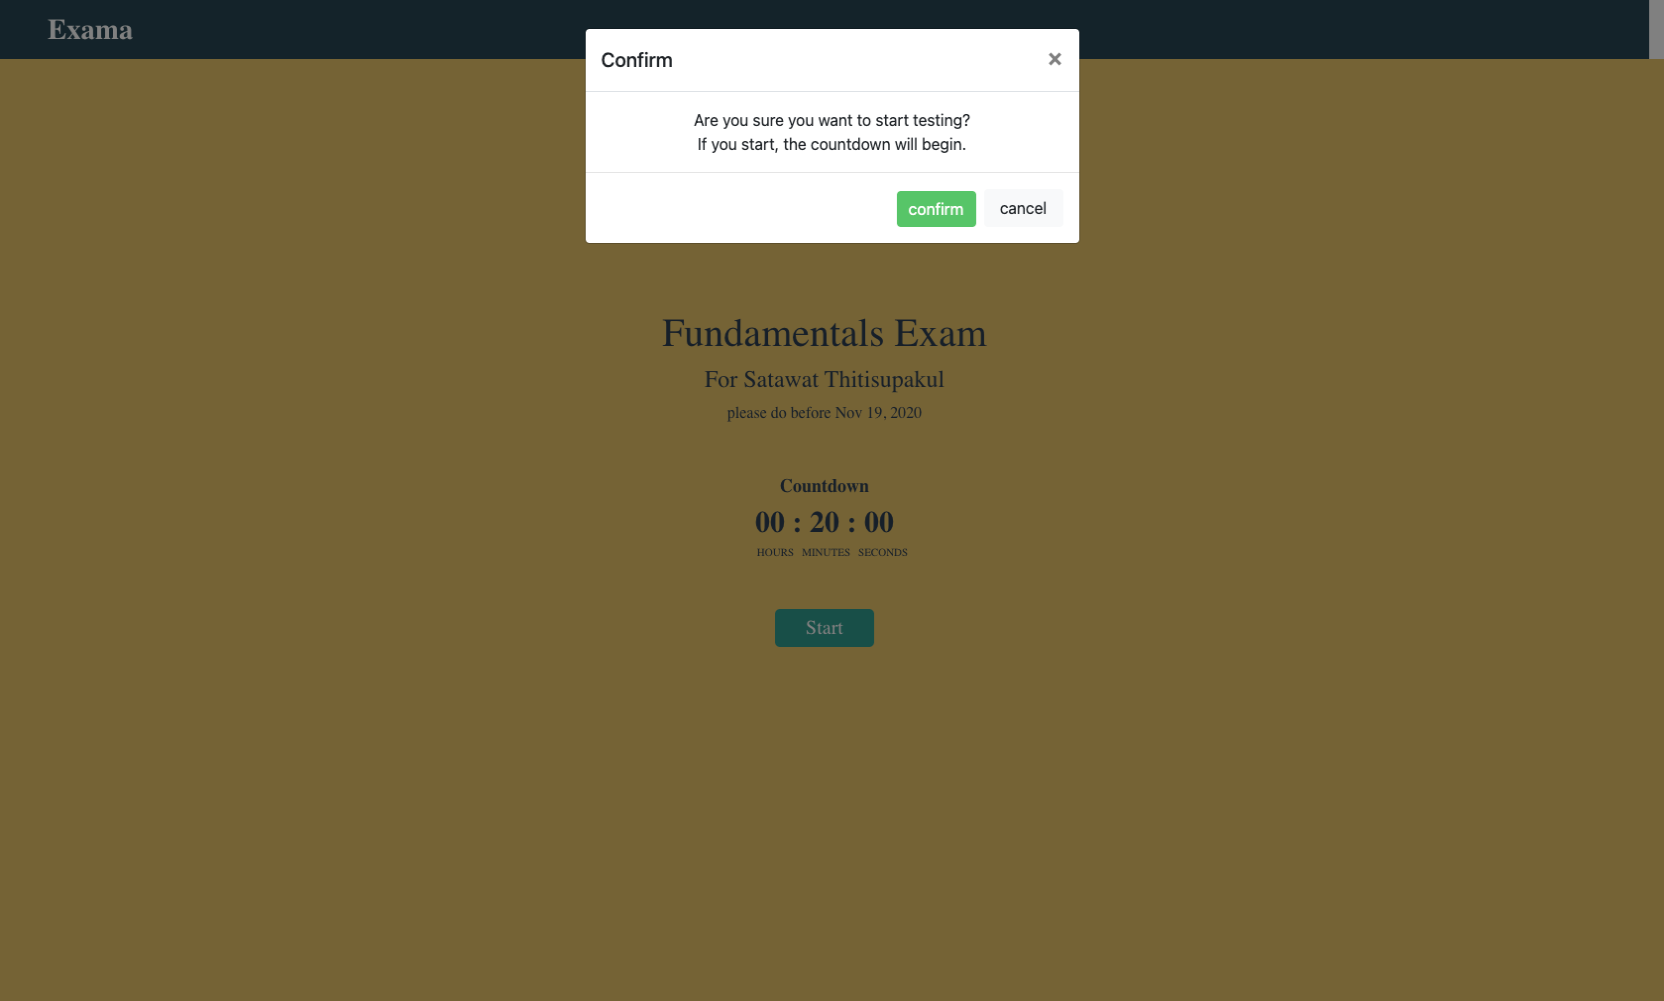
\includegraphics[width=1\columnwidth]{./page/doExam.png}
  \caption{แสดงดูรายละเอียดก่อนเริ่มทำข้อสอบของเว็บแอพพลิเคชั่น}
  \label{Fig:doExam}
\end{figure}
ในหน้าดูรายละเอียดของข้อสอบสำหรับผู้สมัครงานประกอบด้วยฟังก์ชันการทำงานต่างๆ ดังนี้
\begin{itemize}
  \item บอกรายละเอียดต่างๆ ก่อนเริ่มทำข้อสอบ
  \item มีการยืนยันการเริ่มทำข้อสอบ ก่อนที่ระบบจะเริ่มจัดเวลา ดังรูป 4.12
  \item หากข้อสอบหมดอายุ หรือผู้สมัครงานได้ทำข้อสอบนี้ไปแล้ว จะไม่สามารถทำข้อสอบได้
\end{itemize}

\subsection{หน้าทำข้อสอบ}
\begin{figure}[H]
  \centering
  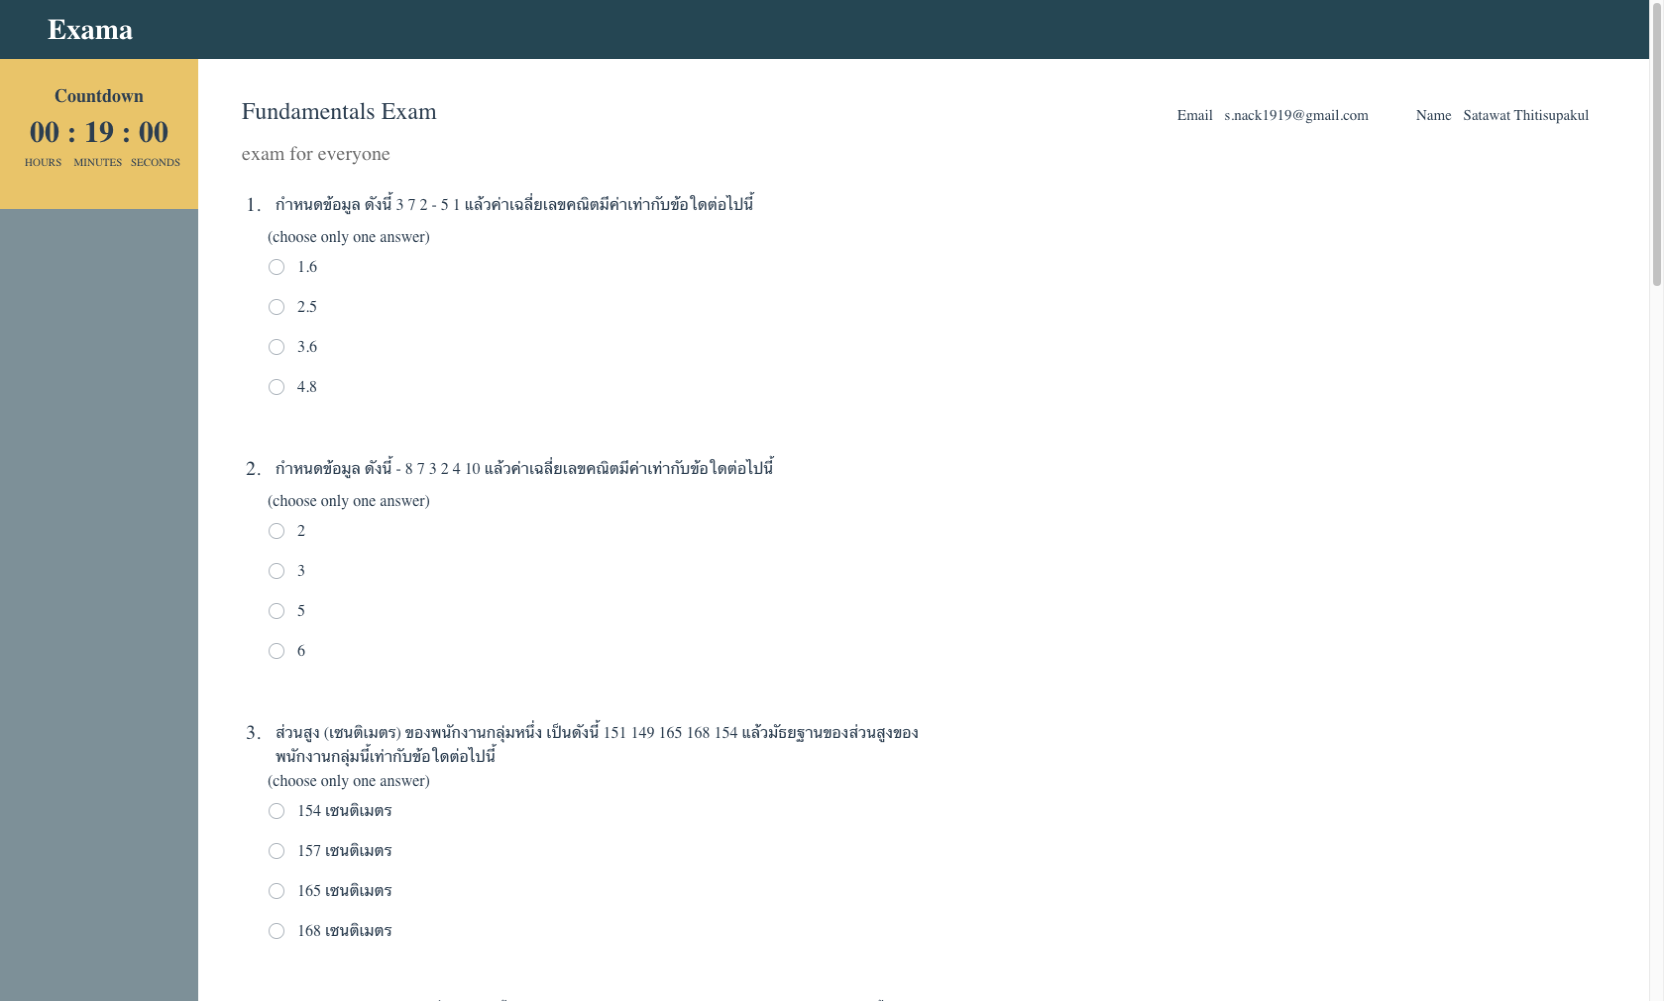
\includegraphics[width=1\columnwidth]{./page/doingExam.png}
  \caption{แสดงหน้าทำข้อสอบของเว็บแอพพลิเคชั่น}
  \label{Fig:doingExam}
\end{figure}
ในหน้าทำข้อสอบประกอบด้วยฟังก์ชันการทำงานต่างๆ ดังนี้
\begin{itemize}
  \item ให้ผู้สมัครทำข้อสอบ
  \item มีการแสดงเวลาที่เหลืออยู่
  \item ผู้ใช้สามารถเข้ามาทำได้ตลอดหากเวลายังไม่หมด
  \item สามารถส่งข้อสอบให้ทางบริษัทได้
  \item หากหมดเวลาสอบแล้วผู้ใช้ยังไม่ได้ส่งข้อสอบให้ทางบริษัท ข้อสอบจะไม่สามารถทำต่อได้และระบบจะทำการส่งข้อสอบให้ทางบริษัททันที
\end{itemize}

\subsection{หน้าแก้ไขข้อสอบเพื่อใช้สำหรับผู้สมัครงาน}
\begin{figure}[H]
  \centering
  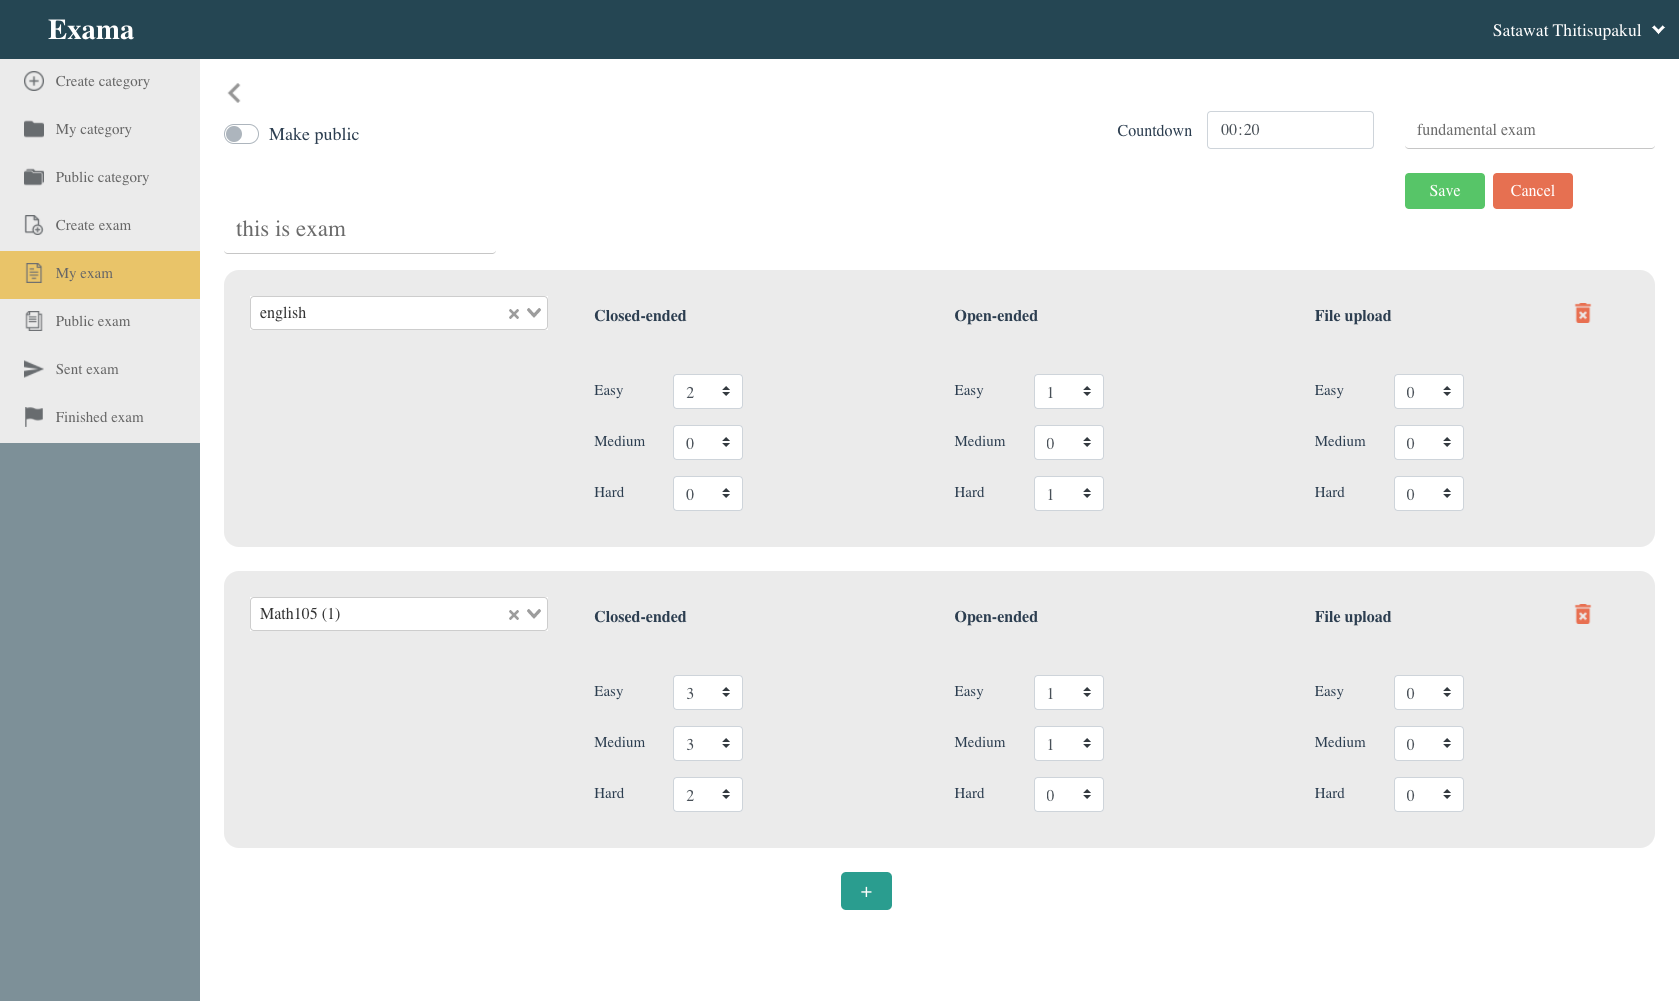
\includegraphics[width=1\columnwidth]{./page/editExam.png}
  \caption{แสดงหน้าแก้ไขข้อสอบเพื่อใช้สำหรับส่งให้ผู้สมัครงานของเว็บแอพพลิเคชั่น}
  \label{Fig:editExam}
\end{figure}
\begin{figure}[H]
  \centering
  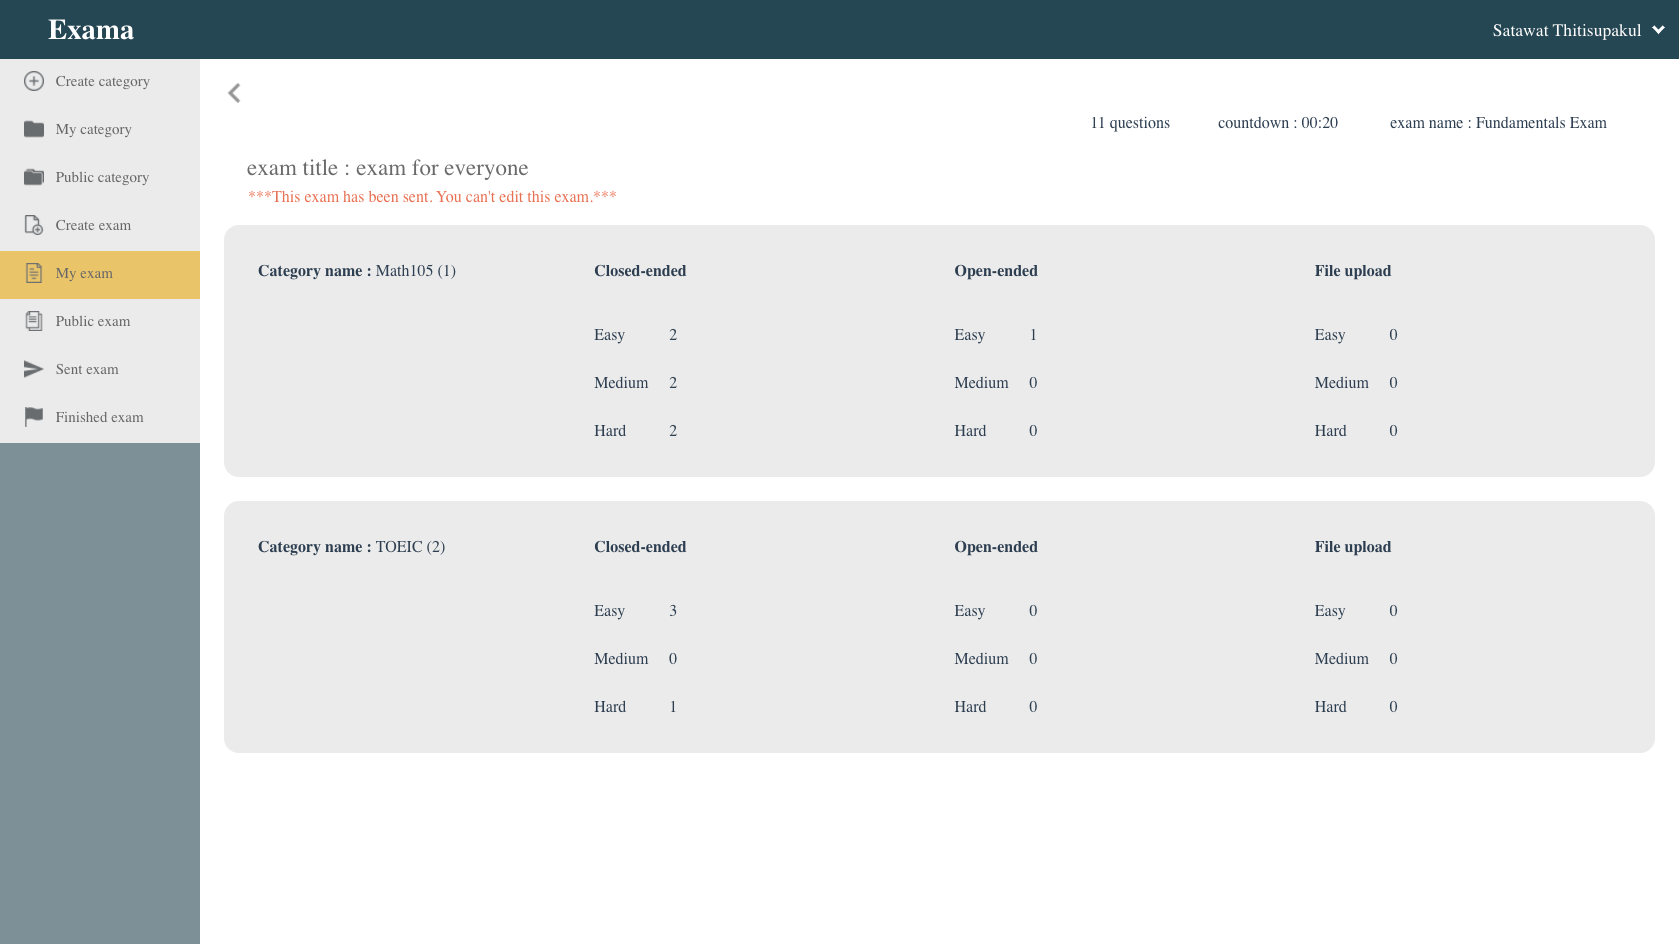
\includegraphics[width=1\columnwidth]{./page/examDetail.png}
  \caption{แสดงหน้าดูข้อสอบเพื่อใช้สำหรับส่งให้ผู้สมัครงานของเว็บแอพพลิเคชั่น}
  \label{Fig:examDetail}
\end{figure}
ในหน้าแก้ไขข้อสอบเพื่อใช้สำหรับผู้สมัครงานประกอบด้วยฟังก์ชันการทำงานต่างๆ ดังนี้
\begin{itemize}
    \item สามารถแก้ไขรายละเอียดต่างๆได้ ดังรูป 4.14
    \item หากข้อสอบถูกส่งไปแล้วจะไม่สามารถแก้ไขรายละเอียดต่างๆได้ ดังรูป 4.15
    \item สามารถป้องกันการกดเปลี่ยนหน้า,การปิดหน้าหรือการรีเฟรชหน้าได้หากผู้ใช้งานทําการป้อน ข้อมูลลงไปแล้ว
\end{itemize}

\subsection{หน้าดูข้อสอบที่เป็นข้อสอบสาธารณะ}
\begin{figure}[H]
  \centering
  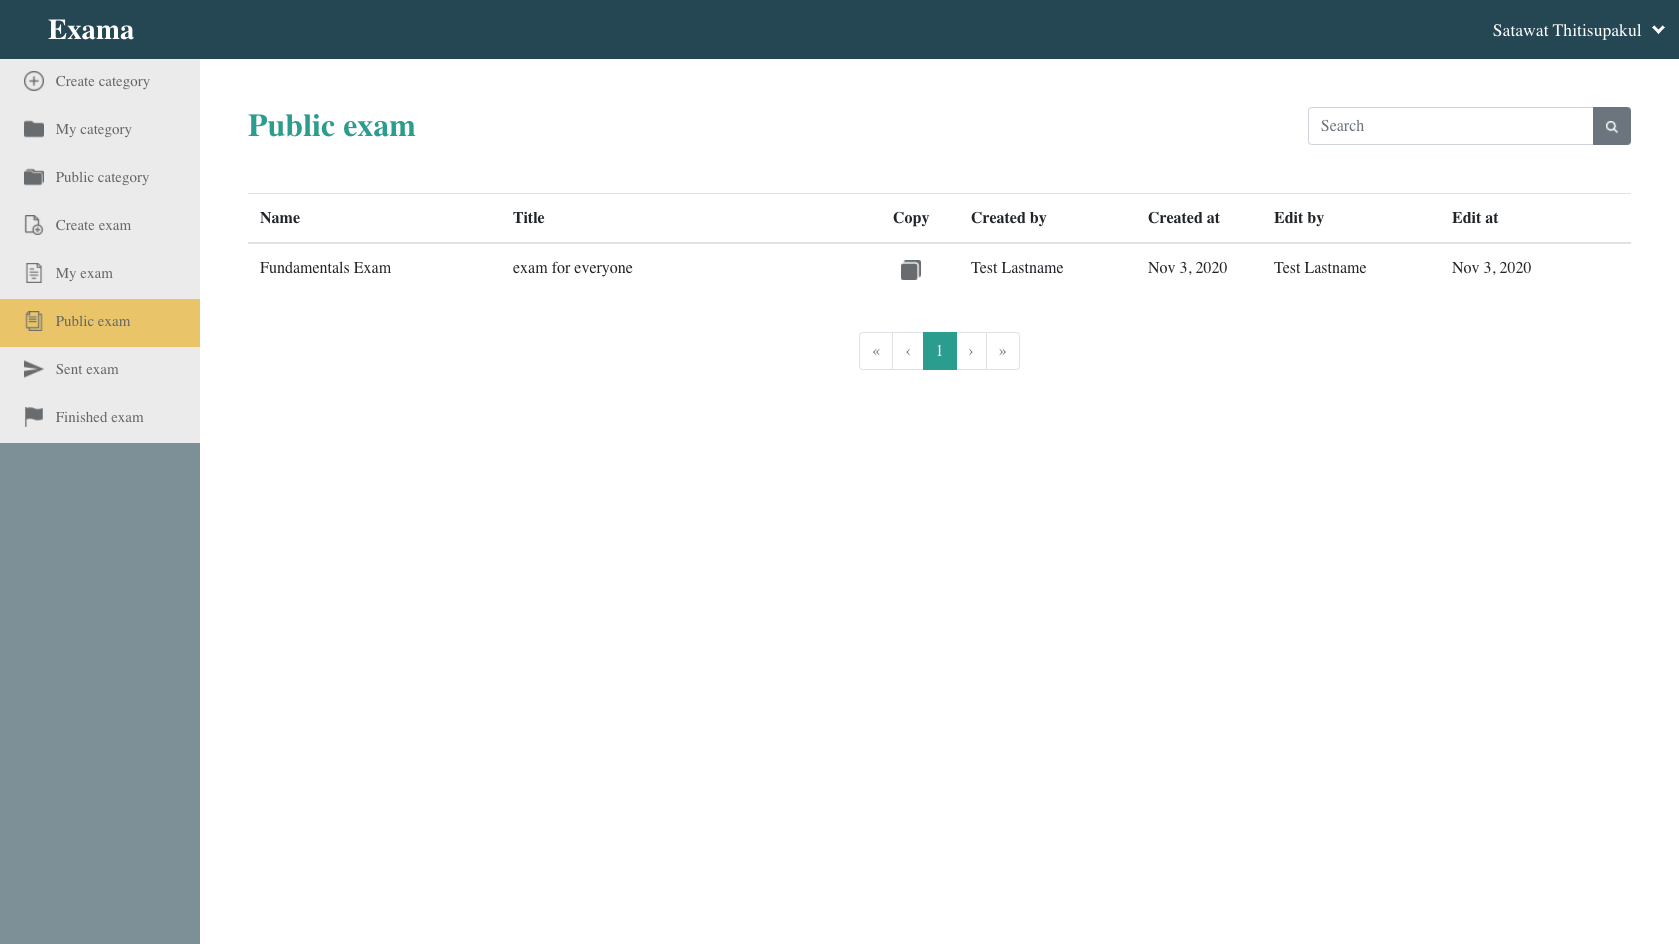
\includegraphics[width=1\columnwidth]{./page/publicExam.png}
  \caption{แสดงหน้าดูข้อสอบที่เป็นข้อสอบสาธารณะของเว็บแอพพลิเคชั่น}
  \label{Fig:publicExams}
\end{figure}
\begin{figure}[H]
  \centering
  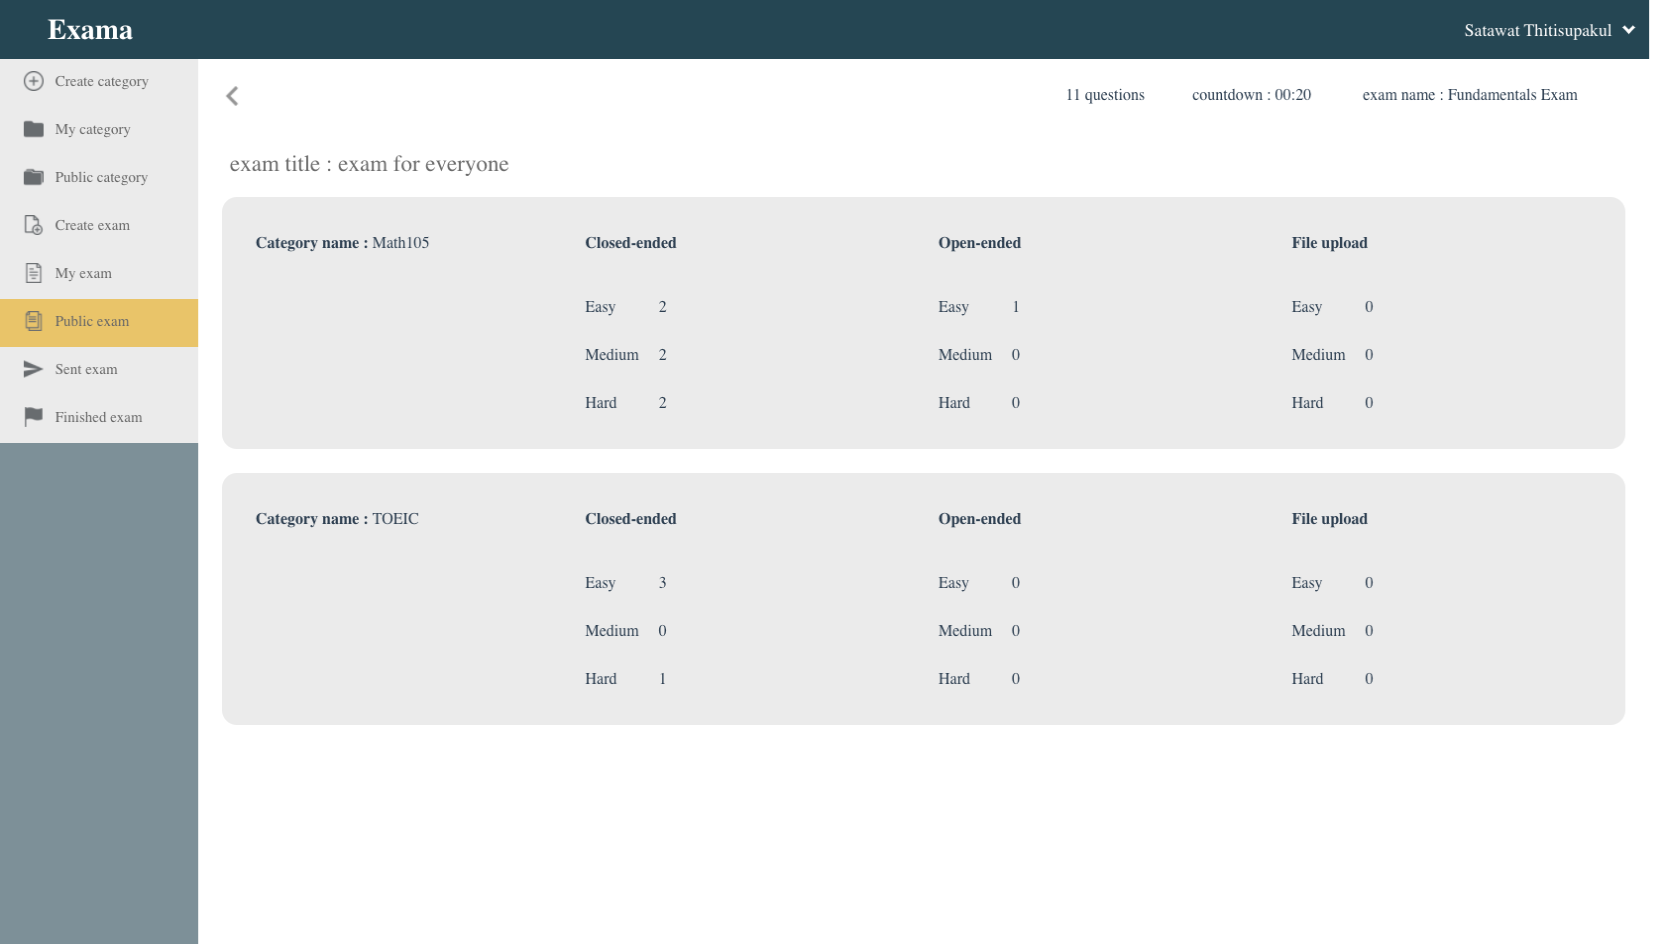
\includegraphics[width=1\columnwidth]{./page/publicExamDetail.png}
  \caption{แสดงหน้าดูรายละเอียดข้อสอบที่เป็นข้อสอบสาธารณะเว็บแอพพลิเคชั่น}
  \label{Fig:publicExamDetails}
\end{figure}
ในหหน้าดูข้อสอบที่เป็นข้อสอบสาธารณะประกอบด้วยฟังก์ชันการทำงานต่างๆ ดังนี้
\begin{itemize}
    \item สามารถดูข้อสอบสาธารณะทั้งหมดได้
    \item สามารถค้นหาข้อสอบที่เป็นสาธารณะได้
    \item สามารถคัดลอกข้อสอบสาธารณะ เพื่อนำมาใช้ หรือแก้ไขได้
    \item สามารถดูรายละเอียดของข้อสอบสาธารณะได้
\end{itemize}

\subsection{หน้าดูประวัติการส่งข้อสอบ}
\begin{figure}[H]
  \centering
  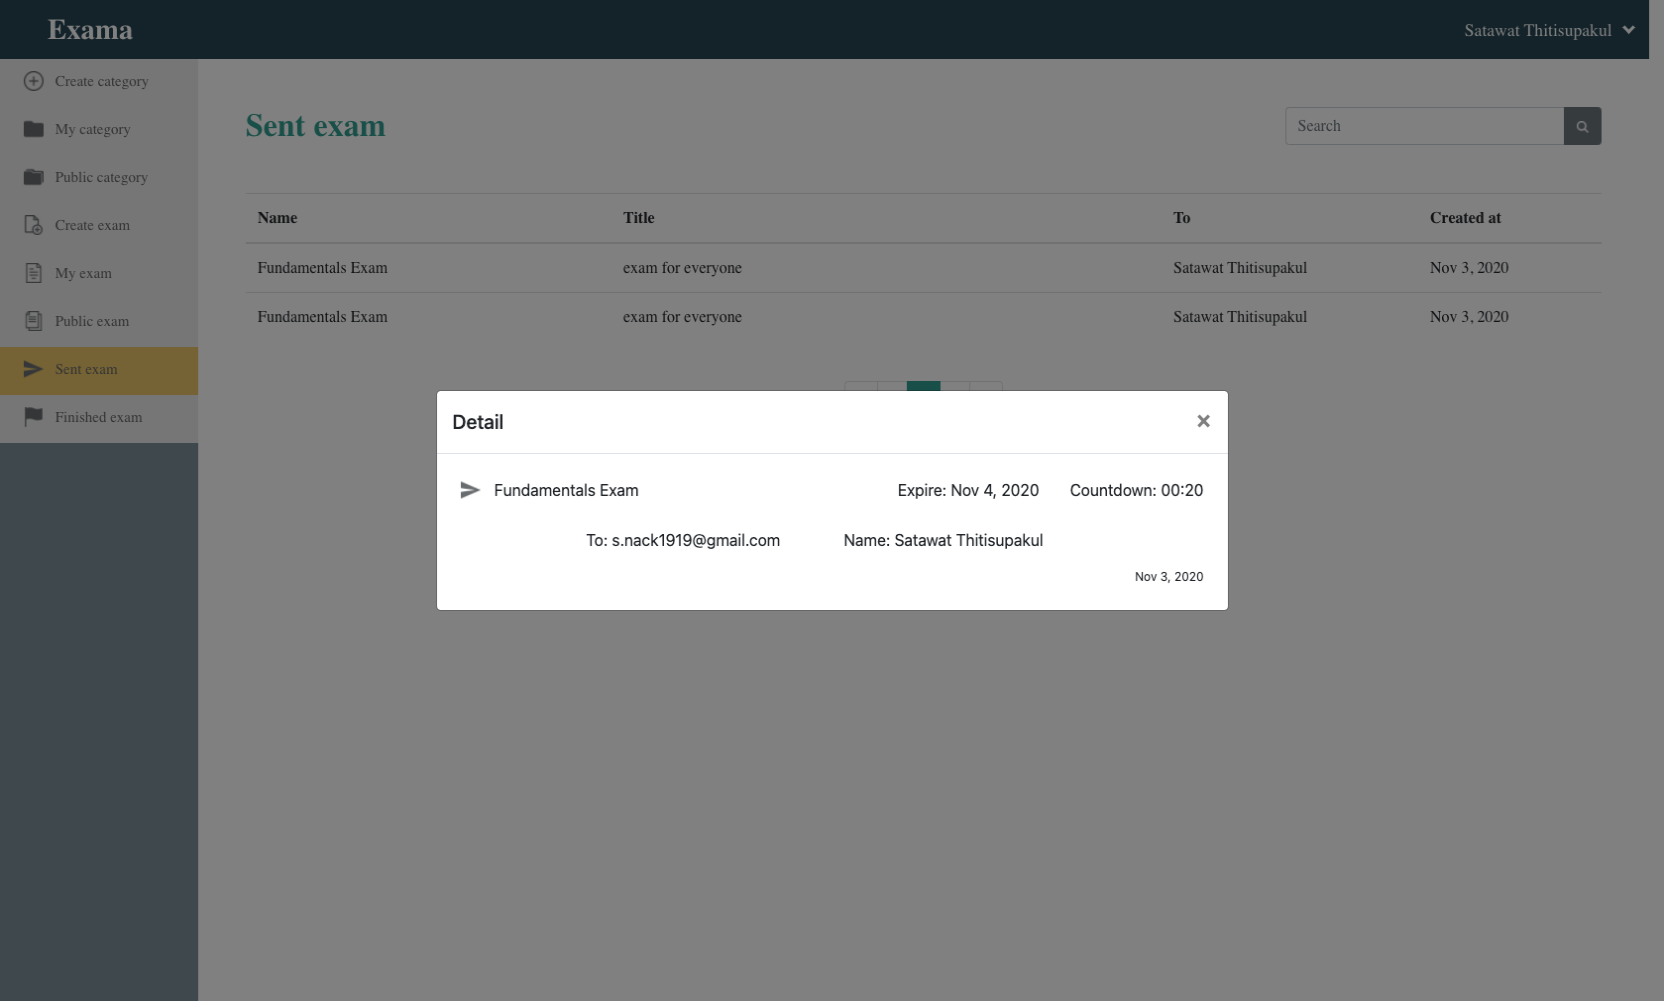
\includegraphics[width=1\columnwidth]{./page/sentexam.png}
  \caption{แสดงหน้าดูประวัติการส่งข้อสอบของเว็บแอพพลิเคชั่น}
  \label{Fig:sentExam}
\end{figure}
ในหน้าสร้างข้อสอบเพื่อใช้สำหรับผู้สมัครงานประกอบด้วยฟังก์ชันการทำงานต่างๆ ดังนี้
\begin{itemize}
    \item สามารถดูรายละเอียดของการส่งข้อสอบได้
    \item สามารถค้นหาประวัติการส่งข้อสอบได้
\end{itemize}

\subsection{หน้าดูข้อสอบที่ผู้สมัครงานทำเสร็จแล้ว}
\begin{figure}[H]
  \centering
  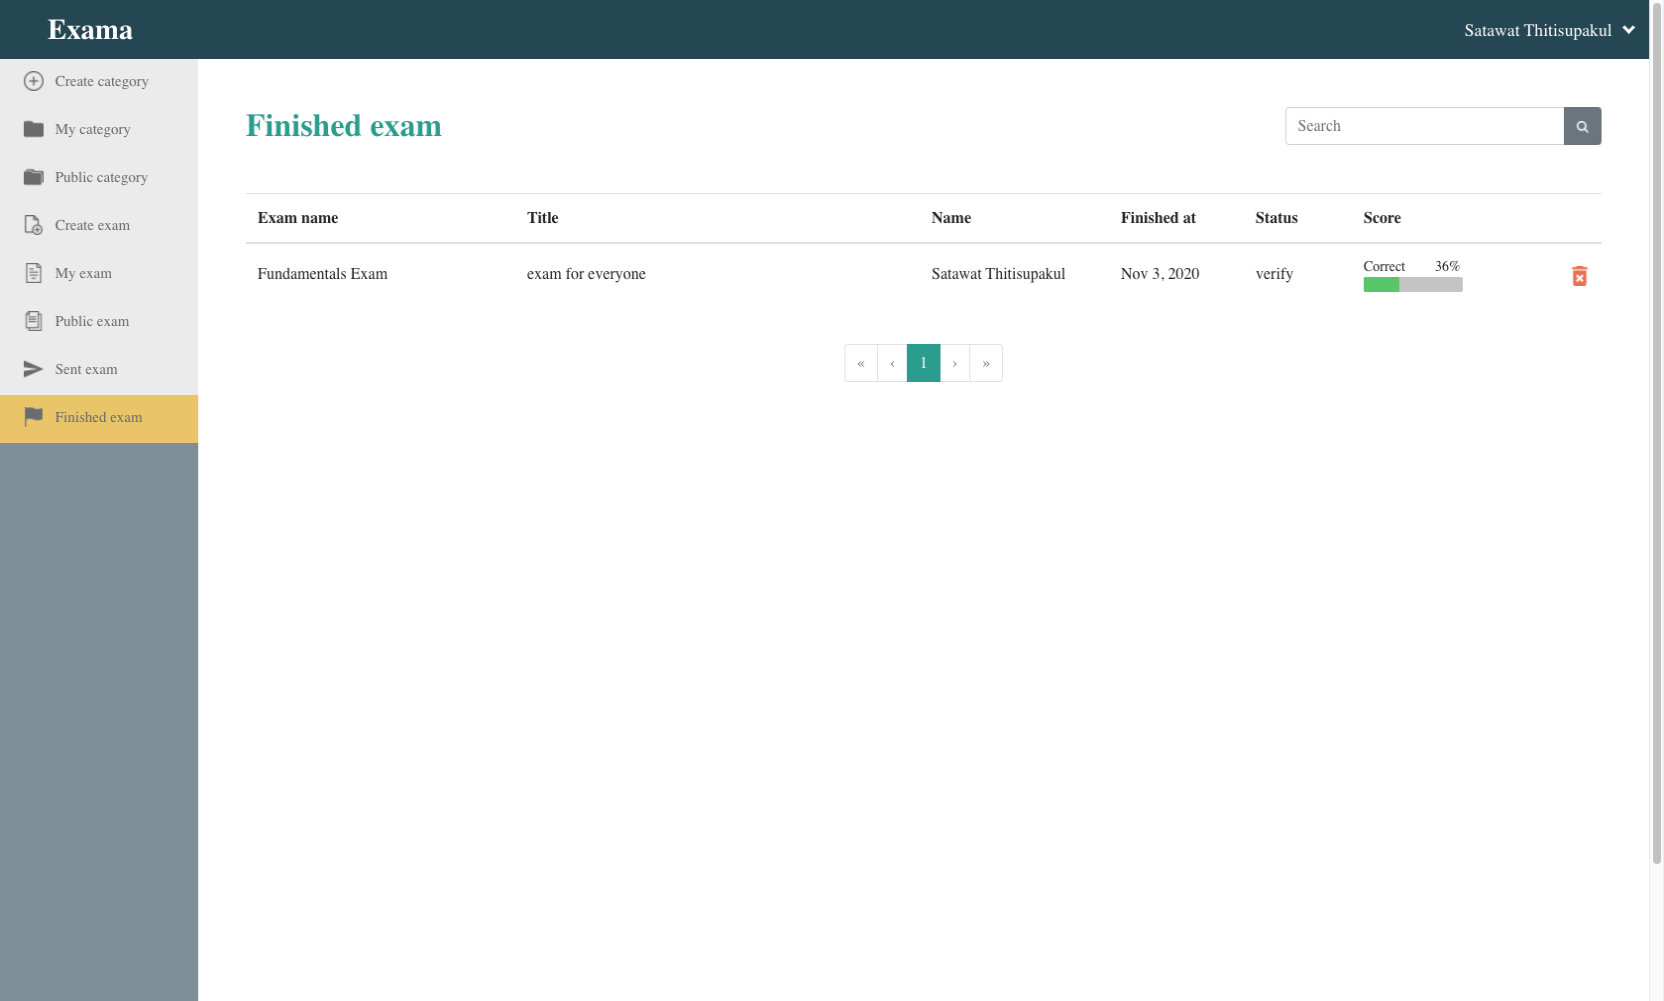
\includegraphics[width=1\columnwidth]{./page/finishedExam.png}
  \caption{แสดงหน้าดูข้อสอบที่ผู้สมัครงานทำเสร็จแล้วของเว็บแอพพลิเคชั่น}
  \label{Fig:finishedExam}
\end{figure}
ในหน้าดูข้อสอบที่ผู้สมัครงานทำเสร็จแล้วประกอบด้วยฟังก์ชันการทำงานต่างๆ ดังนี้
\begin{itemize}
    \item สามารถค้นหารข้อสอบที่ผู้สมัครงานทำเสร็จแล้วได้
    \item สามารถบอกสถานะปัจจุบันของข้อสอบได้ว่าถูก ตรวจโดยพนักงานหรือยัง
    \item สามารถบอกคะแนนของผู้สมัครแต่ละคนได้
    \item สามารถลบได้
\end{itemize}

\subsection{หน้าตรวจข้อสอบของผู้สมัครงาน}
\begin{figure}[H]
  \centering
  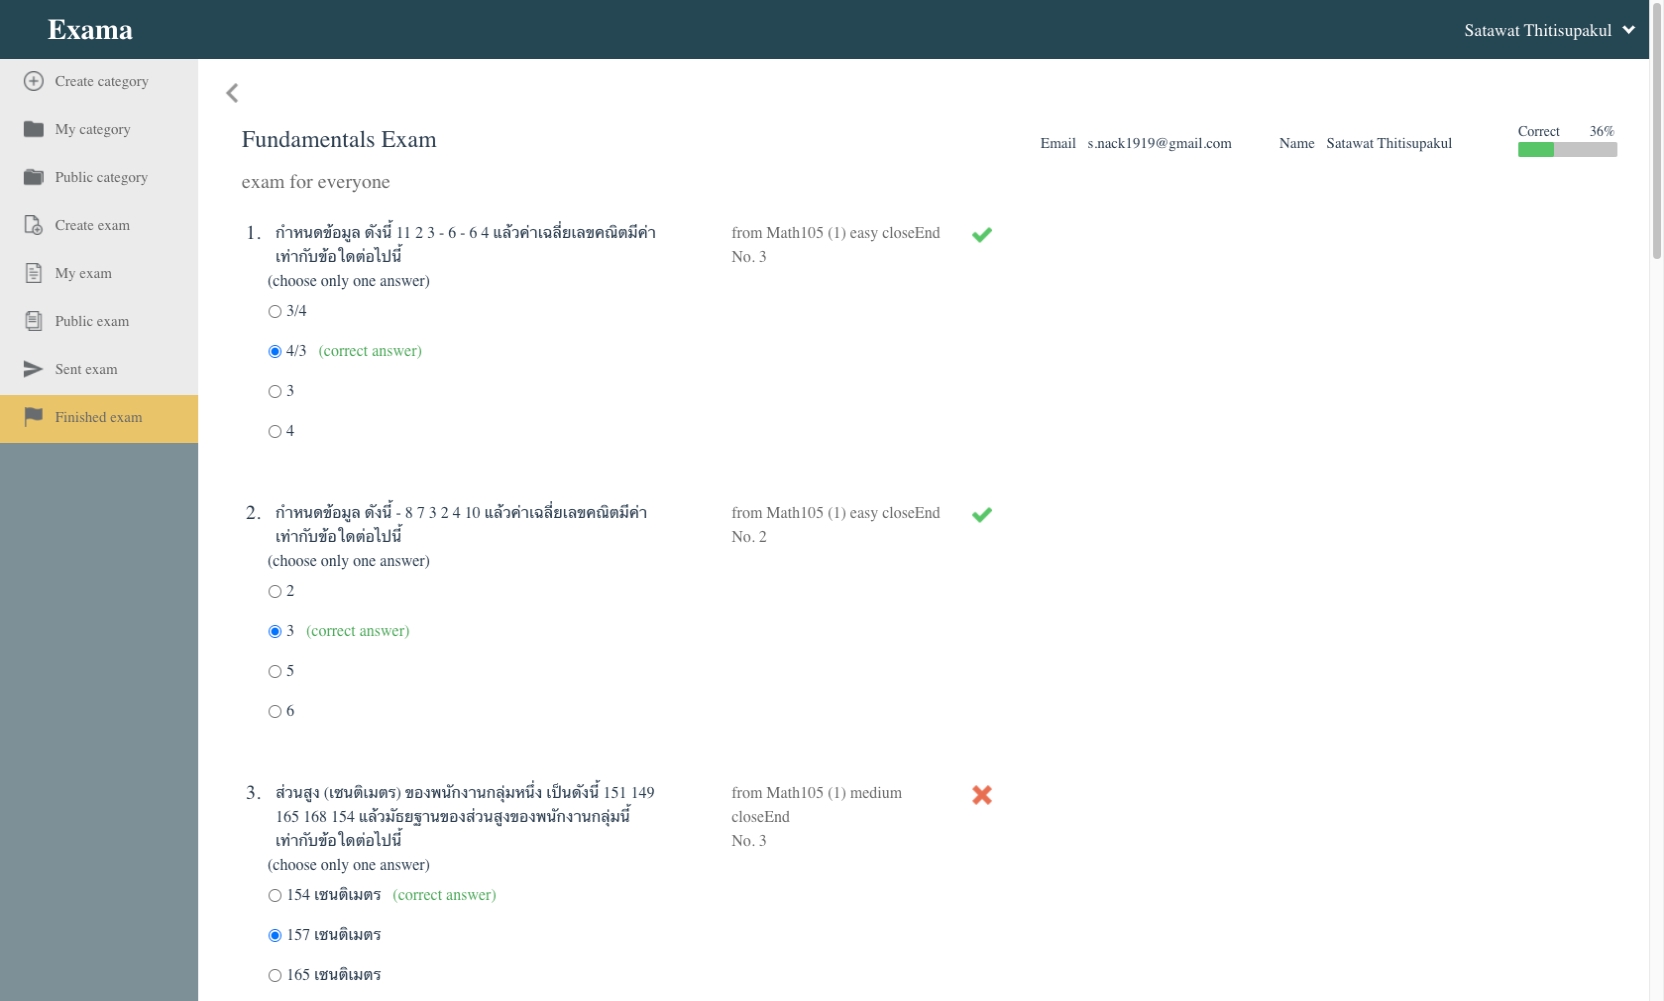
\includegraphics[width=1\columnwidth]{./page/finishedExamDetails.png}
  \caption{แสดงหน้าตรวจข้อสอบของผู้สมัครงานของเว็บแอพพลิเคชั่น}
  \label{Fig:finishedExamDetails}
\end{figure}
\begin{figure}[H]
    \centering
    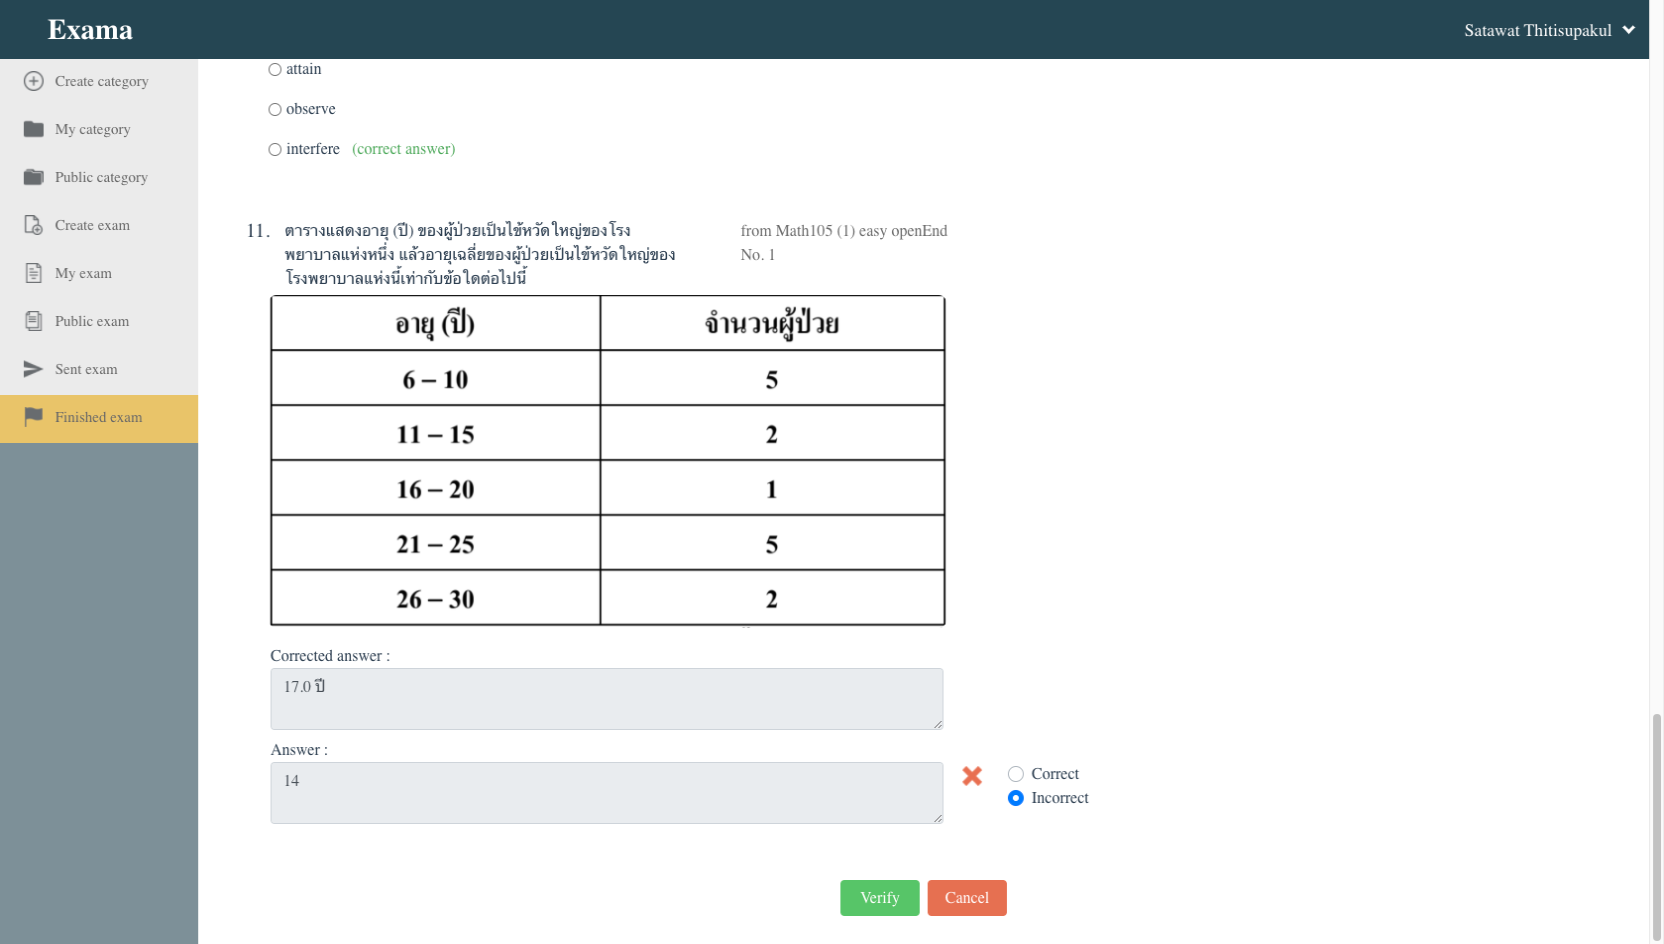
\includegraphics[width=1\columnwidth]{./page/finishedExamDetails2.png}
    \caption{แสดงหน้าตรวจข้อสอบอัตนัยของผู้สมัครงานของเว็บแอพพลิเคชั่น}
    \label{Fig:FinishedExamDetailATN}
  \end{figure}
ในหน้าตรวจข้อสอบของผู้สมัครงานประกอบด้วยฟังก์ชันการทำงานต่างๆ ดังนี้
\begin{itemize}
    \item ระบบทำการตรวจข้อสอบที่เป็นปรนัยแล้วทำการสรุปคะแนนให้โดยอัติโนมัติ
    \item ระบบทำการแสดงคำตอบที่ถูกต้องของคำถามแต่ละข้อ
    \item ระบบสามารถบอกได้ว่าคำถามแต่ละข้อ ถูกสุ่มมาจากหมวดหมู่ไหนและข้อที่เท่าไหร่
    \item ระบบแสดงช่องให้ผู้ใช้ทำการตรวจข้อสอบที่เป็นอัตนัย และข้อสอบที่มีการอัพโหลดไฟล์
    \item สามารถยืนยัน หรือยกเลิกการตรวจได้
\end{itemize}